%% BioMed_Central_Tex_Template_v1.06
%%                                      %
%  bmc_article.tex            ver: 1.06 %
%                                       %

%%IMPORTANT: do not delete the first line of this template
%%It must be present to enable the BMC Submission system to
%%recognise this template!!

%%%%%%%%%%%%%%%%%%%%%%%%%%%%%%%%%%%%%%%%%
%%                                     %%
%%  LaTeX template for BioMed Central  %%
%%     journal article submissions     %%
%%                                     %%
%%          <8 June 2012>              %%
%%                                     %%
%%                                     %%
%%%%%%%%%%%%%%%%%%%%%%%%%%%%%%%%%%%%%%%%%


%%%%%%%%%%%%%%%%%%%%%%%%%%%%%%%%%%%%%%%%%%%%%%%%%%%%%%%%%%%%%%%%%%%%%
%%                                                                 %%
%% For instructions on how to fill out this Tex template           %%
%% document please refer to Readme.html and the instructions for   %%
%% authors page on the biomed central website                      %%
%% http://www.biomedcentral.com/info/authors/                      %%
%%                                                                 %%
%% Please do not use \input{...} to include other tex files.       %%
%% Submit your LaTeX manuscript as one .tex document.              %%
%%                                                                 %%
%% All additional figures and files should be attached             %%
%% separately and not embedded in the \TeX\ document itself.       %%
%%                                                                 %%
%% BioMed Central currently use the MikTex distribution of         %%
%% TeX for Windows) of TeX and LaTeX.  This is available from      %%
%% http://www.miktex.org                                           %%
%%                                                                 %%
%%%%%%%%%%%%%%%%%%%%%%%%%%%%%%%%%%%%%%%%%%%%%%%%%%%%%%%%%%%%%%%%%%%%%

%%% additional documentclass options:
%  [doublespacing]
%  [linenumbers]   - put the line numbers on margins

%%% loading packages, author definitions

%\documentclass[twocolumn]{bmcart}% uncomment this for twocolumn layout and comment line below
\documentclass{bmcart}

%%% Load packages
%\usepackage{amsthm,amsmath}
%\RequirePackage{natbib}
%\RequirePackage[authoryear]{natbib}% uncomment this for author-year bibliography
%\RequirePackage{hyperref}
\usepackage[utf8]{inputenc} %unicode support
%\usepackage[applemac]{inputenc} %applemac support if unicode package fails
%\usepackage[latin1]{inputenc} %UNIX support if unicode package fails


%%%%%%%%%%%%%%%%%%%%%%%%%%%%%%%%%%%%%%%%%%%%%%%%%
%%                                             %%
%%  If you wish to display your graphics for   %%
%%  your own use using includegraphic or       %%
%%  includegraphics, then comment out the      %%
%%  following two lines of code.               %%
%%  NB: These line *must* be included when     %%
%%  submitting to BMC.                         %%
%%  All figure files must be submitted as      %%
%%  separate graphics through the BMC          %%
%%  submission process, not included in the    %%
%%  submitted article.                         %%
%%                                             %%
%%%%%%%%%%%%%%%%%%%%%%%%%%%%%%%%%%%%%%%%%%%%%%%%%


%\def\includegraphic{}
%\def\includegraphics{}
\usepackage{graphicx}



%%% Put your definitions there:
\startlocaldefs
\endlocaldefs


%%% Begin ...
\begin{document}

%%% Start of article front matter
\begin{frontmatter}

\begin{fmbox}
\dochead{Research}

%%%%%%%%%%%%%%%%%%%%%%%%%%%%%%%%%%%%%%%%%%%%%%
%%                                          %%
%% Enter the title of your article here     %%
%%                                          %%
%%%%%%%%%%%%%%%%%%%%%%%%%%%%%%%%%%%%%%%%%%%%%%

%\title{Agenda diversity and coverage bias: A quantitative approach to the agenda-setting theory}
%\title{Agenda setting by comparison of time-evolving topic distribution}
\title{A quantitative analysis of Media Agenda and Public Opinion using time-evolving topic distribution}

%%%%%%%%%%%%%%%%%%%%%%%%%%%%%%%%%%%%%%%%%%%%%%
%%                                          %%
%% Enter the authors here                   %%
%%                                          %%
%% Specify information, if available,       %%
%% in the form:                             %%
%%   <key>={<id1>,<id2>}                    %%
%%   <key>=                                 %%
%% Comment or delete the keys which are     %%
%% not used. Repeat \author command as much %%
%% as required.                             %%
%%                                          %%
%%%%%%%%%%%%%%%%%%%%%%%%%%%%%%%%%%%%%%%%%%%%%%

\author[
   addressref={aff1,aff2},                   % id's of addresses, e.g. {aff1,aff2}
   email={spinto@df.uba.ar}   % email address
]{\inits{SP}\fnm{Sebasti\'an} \snm{Pinto}}
\author[
   addressref={aff3},                   % id's of addresses, e.g. {aff1,aff2}
]{\inits{FA}\fnm{Federico} \snm{Albanese}}
\author[
   addressref={aff1,aff2},                   % id's of addresses, e.g. {aff1,aff2}
]{\inits{COD}\fnm{Claudio O} \snm{Dorso}}
\author[
   addressref={aff1,aff2},                   % id's of addresses, e.g. {aff1,aff2}
   email={balen@df.uba.ar}   % email address
]{\inits{PB}\fnm{Pablo} \snm{Balenzuela}}

%%%%%%%%%%%%%%%%%%%%%%%%%%%%%%%%%%%%%%%%%%%%%%
%%                                          %%
%% Enter the authors' addresses here        %%
%%                                          %%
%% Repeat \address commands as much as      %%
%% required.                                %%
%%                                          %%
%%%%%%%%%%%%%%%%%%%%%%%%%%%%%%%%%%%%%%%%%%%%%%

\address[id=aff1]{%                           % unique id
  \orgname{Departamento de F\'isica, Facultad de Ciencias Exactas y Naturales, Universidad de Buenos Aires}, % university, etc
  \street{Av. Cantilo s/n, Pabell\'on 1, Ciudad Universitaria},                     %
  \postcode{1428},                                % post or zip code
  \city{Buenos Aires},                              % city
  \cny{AR}                                    % country
}
\address[id=aff2]{%                           % unique id
  \orgname{Instituto de F\'isica de Buenos Aires (IFIBA), CONICET}, % university, etc
  \street{Av. Cantilo s/n, Pabell\'on 1, Ciudad Universitaria},                     %
  \postcode{1428},                                % post or zip code
  \city{Buenos Aires},                              % city
  \cny{AR}                                    % country
}
\address[id=aff3]{%                           % unique id
  \orgname{Instituto de Investigaci\'on en Ciencias de la Computaci\'on (ICC), CONICET}, % university, etc
  \street{Av. Cantilo s/n, Pabell\'on 1, Ciudad Universitaria},                     %
  \postcode{1428},                                % post or zip code
  \city{Buenos Aires},                              % city
  \cny{AR}                                    % country
}

%%%%%%%%%%%%%%%%%%%%%%%%%%%%%%%%%%%%%%%%%%%%%%
%%                                          %%
%% Enter short notes here                   %%
%%                                          %%
%% Short notes will be after addresses      %%
%% on first page.                           %%
%%                                          %%
%%%%%%%%%%%%%%%%%%%%%%%%%%%%%%%%%%%%%%%%%%%%%%

\begin{artnotes}
%\note{Sample of title note}     % note to the article
%\note[id=n1]{Equal contributor} % note, connected to author
\end{artnotes}

\end{fmbox}% comment this for two column layout

%%%%%%%%%%%%%%%%%%%%%%%%%%%%%%%%%%%%%%%%%%%%%%
%%                                          %%
%% The Abstract begins here                 %%
%%                                          %%
%% Please refer to the Instructions for     %%
%% authors on http://www.biomedcentral.com  %%
%% and include the section headings         %%
%% accordingly for your article type.       %%
%%                                          %%
%%%%%%%%%%%%%%%%%%%%%%%%%%%%%%%%%%%%%%%%%%%%%%

\begin{abstractbox}

\begin{abstract} % abstract

The mass media plays a fundamental role in the formation of public opinion, either by defining the topics of discussion or by making an emphasis on certain issues. Directly or indirectly, people get informed by 
consuming news from the media. But what are the dynamics of the agenda and how the people become interested in their different topics? 
This  question cannot be answered without proper quantitative measures of agenda dynamics and public attention. 
In this work we study the agenda of newspapers in comparison with public interests  by performing topic detection over the news and identifying the main topics covered and their evolution over time. 
We measure agenda diversity as a function of time using the Shannon entropy and differences between agendas using the Jensen-Shannon distance. We found that the Public Agenda is less diverse than the Media Agenda, especially when there is a very attractive topic and the audience naturally focuses only on this one. Using the same methodology we  detect coverage bias in newspapers and have a first approximation to the theory of framing.
Finally it was possible to identify a complex agenda-setting dynamics within a given topic where the least sold newspaper  triggered a public debate  via a positive feedback mechanism with social networks discussions which install the issue in the Media Agenda.\\

\end{abstract}

%hen there is a very attractive topic, the audience naturally focuses only on this one

%%%%%%%%%%%%%%%%%%%%%%%%%%%%%%%%%%%%%%%%%%%%%%
%%                                          %%
%% The keywords begin here                  %%
%%                                          %%
%% Put each keyword in separate \kwd{}.     %%
%%                                          %%
%%%%%%%%%%%%%%%%%%%%%%%%%%%%%%%%%%%%%%%%%%%%%%

\begin{keyword}
\kwd{agenda-setting}
\kwd{opinion formation}
\kwd{topic detection}
\kwd{mass media influence}
\end{keyword}

% MSC classifications codes, if any
%\begin{keyword}[class=AMS]
%\kwd[Primary ]{}
%\kwd{}
%\kwd[; secondary ]{}
%\end{keyword}

\end{abstractbox}
%
%\end{fmbox}% uncomment this for twcolumn layout

\end{frontmatter}

%%%%%%%%%%%%%%%%%%%%%%%%%%%%%%%%%%%%%%%%%%%%%%
%%                                          %%
%% The Main Body begins here                %%
%%                                          %%
%% Please refer to the instructions for     %%
%% authors on:                              %%
%% http://www.biomedcentral.com/info/authors%%
%% and include the section headings         %%
%% accordingly for your article type.       %%
%%                                          %%
%% See the Results and Discussion section   %%
%% for details on how to create sub-sections%%
%%                                          %%
%% use \cite{...} to cite references        %%
%%  \cite{koon} and                         %%
%%  \cite{oreg,khar,zvai,xjon,schn,pond}    %%
%%  \nocite{smith,marg,hunn,advi,koha,mouse}%%
%%                                          %%
%%%%%%%%%%%%%%%%%%%%%%%%%%%%%%%%%%%%%%%%%%%%%%

%%%%%%%%%%%%%%%%%%%%%%%%% start of article main body
% <put your article body there>

%%%%%%%%%%%%%%%%
%% Background %%
%%

\section*{Introduction}

%\subsection*{Agenda Setting Theory}

\par One of the challenges in  complex social system research is to understand the ecosystem of information flow and opinion formation. 
%Within this framework, many ingredients can be parts of different mechanisms of social influence. 
A major role within this ecosystem is played by the mass media outlets, which are massively used as sources of information.
People get informed by the media and then interact among them via personal discussions or through social networks, giving rise to a complex dynamics where opinions are shaping and changing with time. 
In this scenario, it becomes essential to understand the influence of mass media in a given social group.


% Agenda Setting Theory
\par The influence of the media on public opinion was first explored by the social sciences. 
In the seminal study performed in Chapel Hill during the US presidential elections in 1968 \cite{mccombs1972agenda}, Maxwell McCombs and Donald Shaw found that the aspects of public affairs that are prominent in the news become prominent in the public. This work is considered the founding of the agenda-setting theory.
In its basic stage, known as first-level agenda-setting \cite{mccombs2005look}, the theory focuses on the comparison between the topics coverage by the media and the public agenda, i.e., the topics that the public consider as priority.
For instance, within the agenda-setting framework, it was explored how media content correlate with audiences of different ages \cite{coleman2007young} and how people agendas differ based on the way they consume news \cite{althaus2002agenda}.
On the other hand, the theory hypothesizes how the media affects the audience opinion, in particular, how political coverage and political advertisement shape candidate knowledge among the audience \cite{brians1996campaign, gerber2009does}, or how the coverage given by the media to a particular nation affects people perception about its importance to local political interests \cite{wanta2004agenda}.
Other works examine the differences between public and journalists preferences \cite{mitchelstein2016brecha}, or study the coverage of the main newspapers on particular events related to a confrontation scenario between government and press \cite{zunino2010cobertura, koziner2013cobertura}.

%during the former administration of Argentinian president \emph{Cristina Fern\'andez de Kirchner} (from 2007 to 2015), where the government started to confront with news organizations that were critical to its management \cite{mitchelstein2017information}.

\par The Chapel Hill investigation also induced other several research directions \cite{mccombs2005look}.
One of them focus on detecting media bias, either by taking into account the number of mentions related  to a preferred political party \cite{lazaridou2016identifying, baumgartner2015all} or by identifying the ideology through the position of the media regards to certain issues or actors \cite{elejalde2018nature, sagarzazu2017hugo}. 
This research line can be linked with the theory of \textit{framing} \cite{guggenheim2015dynamics, tsur2015frame}, which focus on the way the media emphasizes some attributes of an object, while understating others. 
On the other hand, several investigations pay attention to the sources of the media agenda, theory known as \textit{intermedia agenda-setting} \cite{vargo2017networks, harder2017intermedia, guo2017global}, where the competition and the mutual influence between different media are observed.

%New trends in agenda-setting theory propose to represent ideological aspects or issues emphasized as networks like mind maps, and the basic idea is the comparison between media's knowledge representative network with its counterpart in the audience \cite{guo2012application, vu2014exploring}.

%\par Nonetheless, most of the works cited above follow typical methods of social science research, and fall in what we call a ``static approach": They used to summarize certain issues present in news media and looking for effects in the audience.
\par Since the irruption of internet, a quantitative analysis based on  the access to big data became available, as for instance, those who takes into account  temporal dependence of the media and public attention. 
In \cite{soroka2017negativity} it is shown that the newspapers and Twitter have an opposite reaction to the changes of the unemployment rates; in \cite{guggenheim2015dynamics}, the competition of frames about gun control is explored; in \cite{ali2018measuring}, the authors show how fluctuations of Twitter activity in different regions depend on the location of terrorist attacks; and in \cite{russell2014dynamics}, the complex interplay between the social media and the traditional one is followed over time on a set of predefined, but general, issues.
However the works cited above have performed a dynamical analysis of agenda-setting based on a single issue or on a set of predefined issues. These are usually  selected by the researcher and use to reflect general subjects, such as ``health" or ``gun control".

% Machine Learning
%by an useful tool employed in the analysis of large documents corpus, but understated in the agenda-setting framework and its derivatives:

\par However, a data driven selection of issues can be performed using a tool frequently employed in the analysis of large document corpus: Unsupervised topic modeling. 
It is an alternative to the dictionary-based analysis, which is the most popular automated analysis approach \cite{guo2016big}, and allows to work with a corpus without a prior knowledge, letting the topics emerge from the data. 
Although many works employ unsupervised topic modeling on news corpus, much of them emphasize the performance of the topic model over a labeled corpus, focusing on the proper detection of the topics \cite{dai2010online, po2016topic, brun2000experiment}. 
In general, issues about the temporal profile of topics are embedded in the context of topic tracking \cite{hu2016news, li2017joint}, or in the recognition of emerging topics in real-time \cite{cataldi2010emerging}, mostly applied to social media. 

\par In this work we propose a novel method in order to study the dynamics of the mass media agenda, which consists of performing an unsupervised topic model on newspapers articles, and studying how the emerging topics evolve with time. 
We look also at their correspondence with the audience agenda, by looking both the Google searches and Twitter activity in the studied period. 
Rather than focus on a single issue or on a set of independent topics, this method allows us to define  the agendas (both the media and the public) as an object which evolves with time.
Our work focuses on a quantitative approach which complements the agenda-setting theory describe above, which mainly stands within the framework of first-level agenda setting, but also allows us to face agenda bias and framing.
We apply this method to study the dynamics of the Argentinian media agenda due to our familiarity with the political background, but as can be seen throughout the work, the methodology implemented is far general and can be easily extended to other datasets. 

\par On the other hand,  new approaches to study social dynamics coming from statistical physics have proposed mathematical models to explore the interplay between the mass media and society \cite{crokidakis2012effects,gonzalez2012model, moussaid2013opinion, rodriguez2010effects, pinto2016setting}. However, much of them lack in being contrasted with real data. 
In this work we are intended to get a closer insight on the complex interaction between the media and the public, and provide a quantitative research in order to construct better and more data-driven models.

\section*{Materials and Methods}
 \label{sec:MatMeth}

\subsection*{The Media Agenda}
\par We analyze a three-month period of the Argentinian media agenda composed by a corpus of news articles that were published between July 31st, 2017 and November 5th, 2017. 
The articles come from the political section of the online editions of the Argentinian newspapers \emph{Clar\'in}, \emph{La Naci\'on}, \emph{P\'agina12}, and the news portal, \emph{Infobae}. The first two lead the sale of printed editions in \emph{Buenos Aires} city, but \emph{Clar\'in} reaches roughly two times the readers of \emph{La Naci\'on}, and ten times the readers of \emph{P\'agina 12} \cite{IVC}, who was chosen because of its left political orientation. On the other hand, \emph{Infobae} has the most visited website, much more than \emph{Clar\'in} and \emph{La Naci\'on} \cite{AlexaAR}.
The corpus analyzed is made up by 2908 politics articles of \emph{Clar\'in}, 3565 of \emph{La Naci\'on}, 3324 of \emph{P\'agina 12}, and 2018 of \emph{Infobae}. Except \emph{P\'agina 12}, all articles were taken from the section \emph{Pol\'itica}  (Politics) of the respective news portals, while the articles which belong to \emph{P\'agina 12} were taken from the section \emph{El pa\'is} (The country).

\par The articles are described as numerical vectors through the \textit{term frequency - inverse document frequency (tf-idf)} representation \cite{xu2003document}. 
Given the set of terms contained in the corpus words, after removing non-informative ones such as prepositions and conjunctions, the \textit{tf-idf} algorithm represents the \textit{i}-document as a vector $v_i = [x_{i1}, x_{i2}, ... , x_{it}]$, where the component $x_{ij}$ is computed by the eq.(\ref{ec:tfidf}), where $\textrm{tf}_{ij}$ is the number of times the \textit{j}-term appears in the \textit{i}-document; $d$ is the number of documents in the corpus; and $n_j$ is the number of documents where the \textit{j}-term appears. 
Each vector is then normalized to unit Euclidean length. 
Once the document vectors are constructed, we put them together in a document-term matrix (\emph{M}), which has dimensions of number of documents in the corpus ($d$) by number of terms ($t$).

\begin{equation}
x_{ij} = \textrm{tf}_{ij} \cdot \textrm{idf}_{j} = \textrm{tf}_{ij} \cdot [1 + \textrm{log}(\frac{1 + d}{1 + n_j})] 
\label{ec:tfidf}
\end{equation}

\par In order to detect the main topics in the corpus, we perform \emph{non-negative matrix factorization (NMF)} \cite{xu2003document, lee1999learning} on the document-term matrix (\emph{M}). A topic is defined as a  group of similar articles which roughly talks about the same subject. 
\emph{NMF} is an unsupervised topic model which factorizes the matrix \emph{M} into two matrices \emph{W} and \emph{H} with the property that all three matrices have no negative elements (see eq.(\ref{eq:nmf})).
This non-negativity makes the resulting matrices easier to inspect, and very suitable for topic detection \footnote{ Even though there are other techniques in topic detection, as for instance LDA (Latent Dirichlet Allocation), the NMF decomposition suites perfect for the kind of corpus we  have analyzed in this work (A detailed comparison of both, NMF and LDA methods could be found in \textbf{Supplementary Material}).}. 
\begin{equation}
M^{(d \times t)} \sim H^{(d \times k)} \cdot W^{(k \times t)}
\label{eq:nmf}
\end{equation}
Such as the resulting matrix \emph{H} has dimensions of number of documents by $k$ and matrix \emph{W} has dimensions of $k$ per number of terms, the number $k$ is therefore interpreted as the number of topics in the documents and it is a parameter that must be set before the factorization.
In this work, we arbitrarily set $k=10$, based on our knowledge of the corpus.
Since the factorization of eq.(\ref{eq:nmf}) usually can not be made exactly, it is approximated by minimizing the reconstruction error, i.e. the distance between matrix \emph{M} and its approximated form $\tilde{M} = H \cdot W$. The \emph{NMF} factorization was made through the python module \emph{scikit-learn} \cite{scikit-learn}.


\par The matrix \emph{H} is the representation of the documents in the topic space. We normalized its rows to unit $l_1$-norm in order to view their components as a degree of membership of a given document in the set of topics. In particular, the index of the largest component tells us which is the most representative topic of the document.
On the other hand, \emph{W} gives the topics representation in the original term space. The largest components of a row give the most representative words of each topic, which we call \emph{keywords}, and therefore an insight of what the topic is talking about.

\par After performing NMF, we represent the time-dependent Media Agenda as a time-evolving distribution of topics. We define $W_i(day)$ to be the daily weight of the topic $i$, which is calculated following the eq.(\ref{eq:topic_weight}), where $l(j)$ is the number of words of the document $j$; $h_{ji}$ is the degree of membership of document $j$ on topic $i$; $d_j$ is the date of document $j$; and $\delta$ is the Kronecker delta. 
Providing by the fact that each document vector can have all non-zero components, it is allowed that a document contributes to more than one topic weights.
In order to reduce noise, we apply a linear filter with a three day wide sliding window, and finally we normalize the temporal profiles in order to describe each newspaper agenda as a distribution over the topic space, which evolves over time. 
%This last normalization prevent us against the differences in the number of articles that each newspaper publishes.

\begin{equation}
W_i(day) = \sum_j l(j) \cdot h_{ji} \cdot \delta_{d_j,day}
\label{eq:topic_weight}
\end{equation}

\subsection*{The Google and Twitter Agendas}
 
\par Besides the construction of the Media Agenda it is important to have some measure of the public interests and construct what we call the Public Agenda. 
To achieve this goal, we take Google and Twitter as proxies of the public interests by looking for the same topics in the same period of time. We take advantage of the topic keywords in order to make queries into the \emph{Google Trends} tool and into the advance search tool of Twitter, and therefore we get the relative weight of searches and tweets in each respective platform. 
In this way, the Public Agenda is described, in an independent way, by the Google and Twitter Agendas. 
In section \textbf{Results} we will give a more detailed description of the keywords involved in their construction.

\subsection*{Normalized Shannon Entropy ($H$)}

\par In fact, one of the key of our work is the representation of the Agendas as time evolving topic distributions, and the association between the different measures that we can derive from them with the social events observed during the period.
In order to do that, we focus in the concept of \emph{diversity of the attention}.
\emph{Diversity} is a very important variable that must be taken into account when dealing with multiple issues \cite{boydstun2014importance}, due to the fact that it tells us how the attention is distributed across the different topics of discussion. 
As was proposed in \cite{boydstun2014importance}, we use the normalized Shannon entropy to quantify the diversity within our framework.
\par The normalized Shannon entropy $H[p]$ referred in eq.(\ref{eq:shannon_entropy}) gives us a measure of how spread is a -discrete- distribution, taking the maximum value of $1$ when all outcomes are equally probable (as in the case of having a diverse agenda), and $0$ when there is just one possible outcome (when one topic of discussion dominates the agenda). 
%This last case, or an approximated one, will be of particular interest for us because it tells about a topic which absorbs all the attention either from the Media or the Public, while the former shows an absolutely unbiased interest towards any of the topics.

\begin{equation}
H[p] = \frac{- \sum_{i = 1}^{N} p(x_i) * ln(p(x_i))}{ln(N)}
\label{eq:shannon_entropy}
\end{equation}

\subsection*{Jensen-Shannon distance}

\par While the diversity is a property of each distribution, a natural question that arises when comparing different distributions is how similar they are. For instance, we will be particularly interested in measuring the similarity between the Media and Public Agendas, because lower values would indicate distant interests between the media and its audience.
We measure the similarity between distributions via the Jensen-Shannon distance ($JSD$). 
When the similarity of the distributions is low, the distance between them is high.
\par The Jensen-Shannon distance ($JSD$) is a metric between distributions based on the Jensen-Shannon divergence ($JS_{Div}$) \cite{fuglede2004jensen}, which is in turn a symmetric version of the well-known Kullback-Leibler divergence $D_{KL}$ (eq.(\ref{eq:kl})). 
We recall that the $JSD$ has the advantage of being symmetric and also a well-defined distance, which makes it conceptually easier to deal with.
As can be seen in eq.(\ref{eq:jensen_shannon_distance}), the $JSD$ between the distributions $P$ and $Q$ is simply the square root of the Jensen-Shannon divergence, where $M = \frac{P + Q}{2}$.

\begin{equation}
D_{KL}(P||Q) = -\sum{P(i) log(\frac{Q(i)}{P(i)})}
\label{eq:kl}
\end{equation}

\begin{equation}
\label{eq:jensen_shannon_distance}
JSD(P,Q) = \sqrt{JS_{Div}(P,Q)} = \sqrt{\frac{1}{2}[D_{KL}(P||M) + D_{KL}(Q||M)]} 
\label{eq:jensen_shannon_distance}
\end{equation}

\subsection*{Outliers identification}

\par As was mentioned before, once the concepts of diversity and distance between distributions were defined, we are particularly interested in those dates when these measures take extreme values: Lower values of diversity indicate a topic which is absorbing much of the attention of any of the Agendas; on the other hand, when the distance between two distributions is high, we can conclude that they have distant interests.
However, we still lack the definition of what a low diversity or a high distance are. 
We face this problem by treating the measures of each observable as random samples from a population with unknown distribution, and identifying those extreme values as outliers of the distribution. 
In order to detect these outliers we follow the popular box-plot construction proposed by Tukey \cite{tukey1977exploratory}, which is a simple data-driven method and has the advantage of making no prior assumption about the distribution of the data. 
However, it is important to remark that the constants involved in the outliers definition (see eq.(\ref{eq:fences})) is taken from applying this method on a normal distribution.
\par In the box-plot construction a quartile division of the $N$ observations is proposed. We name $Q1$ as the lower quartile, $Q2$ the median of the distribution, and $Q3$ the upper quartile. Recall that $Q1$ ($Q3$) is defined to be the division where the 25th (75th) percent of the observations lies below (by definition, the median $Q2$ separates the distribution in two equal parts). On the other hand, the inter-quartile range $IQ$ is defined to be $IQ = Q3 - Q1$. This is the range where the bulk of the data lies inside.
We are not interesting in the visualization of the box-plot in its own but instead in its procedure to identify outliers. Therefore, from the identification of the quartiles, new quantities called \emph{fences} are defined in eq.(\ref{eq:fences}): The \emph{lower inner fence} ($LIF$), the \emph{upper inner fence} ($UIF$), the \emph{lower outer fence} ($LOF$), and the \emph{upper outer fence} ($UOF$). The fences can be interpreted as the limits of the distribution.
\begin{eqnarray}\label{eq:fences}
LIF & = Q1 - 1.5 IQ \nonumber \\
UIF & = Q3 + 1.5 IQ \nonumber\\
LOF & = Q1 - 3 IQ \nonumber \\
UOF & = Q3 + 3 IQ
\end{eqnarray}
\par We then have all the ingredients to label a point as an outlier: A point which lies above the upper inner fence is considered a \emph{mild outlier}, while a point that lies above the upper outer fence is considered an \emph{extreme outlier}. The same holds for the lower fences, i.e. if a point lies below the lower inner (outer) fences is considered as a mild (extreme) outlier \cite{natrella2010nist}. 
We will indicate the proper fences in each figure either when the diversity or the distance is being analyzed. We will pay attention not only to those values labeled as outliers, but also to those that are next to any of the fences despite not being strictly defined as that.

\section*{Results}
\label{results}

\par We initially focus on the ten most important issues from the three-month period corpus of news reported above. 
The election of factorizing the corpus in ten topics was based on having a low dimensional representation of the corpus and a clear interpretation of the topics due to our prior knowledge of the political background. 
We found that this factorization allowed us to draw useful conclusions. However, more sophisticated methodologies to estimate the number of topics in a corpus can be taken into account in future researches.
The ten topics are represented in the word clouds of figure \ref{fig:topics_wordclouds}.
Given our interpretation of the keywords found in three of them, we joined these topics as being part of the same macro-topic which we called \emph{Elections}.
On the other hand, the same holds for other two topics which were classified as part of a macro-topic called \emph{Missing person}. 
Therefore, the ten original topics were reduced to seven, which are pointed out in the radar plot of figure \ref{fig:topics_wordclouds}.
The meaning of the topics or macro-topics is contextualized in the \textbf{Supplementary Material}.
\par Finally, by following the procedure described in the previous section, we construct the \textbf{Media Agenda (MA)} and the \textbf{Public Agenda (PA)}, in both its Google and Twitter derivations, as time-evolving distributions in the space of seven topics.

\subsection*{The Media and Public Agendas}

\par In figure \ref{fig:topics_wordclouds} we show a seven topic decomposition of the whole corpus using radar plots for the Media \textbf{MA} and Public agendas \textbf{PA} discriminated by \textbf{GT} (Google Trends) and \textbf{Tw} (Twitter). In this figure we also show the word clouds of the keywords that define each of the ten original topics, where the size of the word reflects its importance in the topic definition. In green color, we point out the words involved in the Google Trends and Twitter queries in order to construct the Public Agenda. The queries employed are also specified in tables \ref{table:gt_queries} and \ref{table:tw_queries}. 
On the other hand, in table \ref{table:gt_all_correlation} we show the linear correlation between the topic temporal profiles from the Public Agenda and their counterparts in the Media Agenda.
\par We can see that both GT and Tw look similar in this representation, but they show specific differences with the Media Agenda. For instance, a greater interest of the audience in the topic \emph{Missing person} than the media is observed, or inversely, a lower interest in the topic \emph{Prosecutor's death} takes place. However, this static representation is not able to show the complex dynamics of the agendas evolution and the importance of punctual and specific facts which can erase or amplify their differences. 

\par The time evolution of the topics is shown in a bump chart of the Agendas by figure \ref{fig:all_agenda}. The bump chart provides  a clear visualization of the relative weight of the topics at the same time with their ranking. In figure \ref{fig:all_agenda}, we also highlight some important events related to the dynamics of the topics.
It is possible to appreciate how the main topic changes with time and have a glance of the qualitative differences between the agendas. In particular, it can be seen some differences between the Public Agendas that were not observed in figure \ref{fig:topics_wordclouds}, as for instance, the persistence of main topics is longer in Twitter than in Google Trends. This is more evident at the end of the analyzed period, where the topics discussed in Google Trends show more response to change in Media Agenda than in Twitter, maybe due to the existence of a different pattern of interaction in the social network, to which a deeper analysis could be devoted in future works.
\par The linear correlations between the same topics of MA and PA were also calculated. In all cases, we found that the correlations are positive and statistically significantly, as it is shown in table \ref{table:gt_all_correlation}.  
We interpret this as a validation of the topics found in the corpus and the keywords that describe it. Even though we are particularly interested in those periods where the Agendas differ, it is expected that the media and public interests should generally follow a similar a pattern, mainly driven by external events
A non positively (or a non significantly) correlation may imply, besides the obvious conclusion of agendas disengagement, that we can be eventually failing to properly detect the keywords or features that describe a particular topic, and therefore the comparison of the Google Trends or Twitter patterns with their counterpart in the Media Agenda would be wrong.

%\par The figures introduced above show not only the topics and their differences between the Agendas, but also the dynamics of the topics.  For instance, we can see in the radar plot of figure \ref{fig:topics_wordclouds}, a greater interest of the audience in the topic \emph{Missing person} than the Media, or inversely in the topic \emph{Prosecutor's death}, at least in the analyzed time-lapse. We can also observe a great similarity between \textbf{GT} and \textbf{Tw} agendas which both are different faces of the Public Agenda.

\subsection*{A quantitative description of the Agendas}

\subsubsection*{Agenda diversity}

\par How dominant is a main topic? Is the degree of dominance of a given topic in the Media Agenda reflected in the Public Agenda? In order to answer such kind of questions we quantify the diversity of the agendas through the normalized Shannon entropy $H$, which was introduced in section \textbf{Material and Methods}.
\par In figure \ref{fig:shannon_entropy_agendas} we can see the value of $H$ as a function of time for the three agendas. It is important to pay attention to those periods of time when the diversity is lower than usual. This effect is notoriously more pronounced in the Public Agenda giving by GT, and in particular in four specific days when four local minimums of the Shannon entropy can be detected. Three of them are outliers as defined in section \textbf{Material and Methods}, two of them from GT and one from Tw. The other one has been not identified as an outlier but it is a pronounced minimum and therefore a point of interest in our description. 
 
\par A lower value in the agenda diversity is due to the fact that the most important topic attracts practically all the attention of the public and the media, collapsing the agenda to one of the issues involved.
In the radar plots included in figure \ref{fig:shannon_entropy_agendas} we can see how two of these outliers (\textbf{a} and \textbf{d}) belong to the topic \emph{Elections}. They are related to the primary and general legislative elections that took place in August 13th and October 22nd respectively.
In all the agendas these points were detected as outliers except point (d) in Twitter Agenda. Why is that? The radar plot of the Twitter agenda for this day displays an association between the topic \emph{Elections} and the \emph{Current President}, decreasing the importance of this topic.
Discussions in Twitter about elections appear also in point (c), when the other agendas seem to be more diverse. 
On the other hand, and despite not being classified as outlier, we also focus on point (b) because the Shannon Entropy in the Google Agenda displays a minimum (collapsing agenda) which is not corresponded neither in the Media nor in the Twitter Agendas. Crawling in the context, we see that it belongs to the topic \emph{Missing person} and this date corresponds to the rally that took place one month after the disappearance of \emph{Santiago Maldonado} (see \textbf{Supplementary Material}). 
We  would like to emphasize the discussion about this topic (\emph{Missing person}) because its dynamics show interesting features, as we will show below.

\par From the measure of $H$ we have also observed that the median of the Public Agenda diversity is statistical significant lower than the median of the Media Agenda.
Specifically $H_{GT} = 0.73$ and $H_{Tw} = 0.74$ are statistically significantly lower than $H_{MA} = 0.85$ with $p < 10^{-18}$, while there is no significant difference between the first two. 
However, from figure \ref{fig:shannon_entropy_agendas} we can see that GT shows more abrupt dropouts in the diversity in response to specific events.
From all this analysis we  can conclude that given a finite set of topics, \textbf{the Public Agenda is less diverse than the Media Agenda}, because the public seems to focus on the most important topics than the media can do, maybe due to editorial decisions.

\subsubsection*{Distance between Media and Public Agendas}

\par Given our descriptions of the agendas as time-evolving distributions, we can  compare them by computing the Jensen-Shannon distance. In this context, outliers in selected dates will correspond to divergences between the Media and Public Agenda: Specific events when the public interests do not match with media offer.
In figure \ref{fig:jensen_shannon_gt} we show the Jensen-Shannon distance between Media and Public Agendas as a function of time. We focus on three points that seem to be relevant enough. In all cases, the topic distributions at these days displayed show that the increment in the distance between agendas is due to a greater interest of public opinion in the \emph{Missing person} topic. 

\par Points \textbf{(c)} and \textbf{(d)} show that both the public and the media highlight this topic, but the media do not disregard other topics, so the corresponding distance between them can be interpreted as lack of diversity in Public Agenda as discussed in the last section.

\par On the other hand,  points \textbf{(a)} (we take this point due to be a local maximum despite not being an outlier) and \textbf{(b)}  show a major  interest of the public in the topic \emph{Missing person} which it is not reflected in the Media.  
In figure \ref{fig:all_agenda} we can see that this topic becomes the most important in public interests (both in GT and Tw) days before that it happens in the Media Agenda. This fact can be associated  with a social networks (like Facebook and Twitter) campaign  in favor  of the appearance of \emph{Santiago Maldonado} (``The missing person") that took place on  August 26th. This campaign was massive and  initially underestimated by the main media outlets in Argentina (see \textbf{Supplementary Material}). 

\par % It is important to notice that it is our interpretation of the data based on the knowledge of the context, and  we are not measuring causality between Agendas (we will say a few words about it in section \ref{sec:who_sets}), i.e. we can't say, for instance, that in this case the Public Agenda set the Media Agenda. 
Finally, it is important to say that the Jensen-Shannon distance, together with the measurement of agenda diversity given by the Shannon entropy, give an insight of independent behavior, in certain particular dates,  of the public and the media. Its identification can be a starting point to study the media reaction to a change in audience interests.
 
\subsection*{Agenda bias in different media outlets}

\par In this section we leave aside the Public Agenda as an unified corpus and we study the composition and evolution of the Media Agenda on each media outlet. 
In figure \ref{fig:news_agenda} we show the bump charts corresponding to each of the analyzed newspapers analogously to figure \ref{fig:all_agenda}.
The topics are the same which were introduced in the word clouds of figure \ref{fig:topics_wordclouds}, but when computing the topic weights, the articles are discriminated by newspaper. 
We also show the radar plots with the average distribution, as made in figure \ref{fig:topics_wordclouds}. 

\par In figure \ref{fig:news_agenda} we can qualitative look at the differences between the newspaper agendas.
For instance, we can see how the newspaper called \emph{P\'agina 12} gave more importance to the topics \emph{Missing person} and \emph{Social leader}, while it reduces to minimum the coverage of the topic  \emph{Former Planning minister} as the others did.

\par In order to detect significant bias coverage of a given newspaper, we again calculate the Jensen-Shannon distance, but between the individual newspapers agenda and the Media Agenda.
Note that this is the distance between the distributions of figure \ref{fig:news_agenda} and the top panel of figure \ref{fig:all_agenda}. 
 In figure \ref{fig:jensen_shannon_news} we show the Jensen-Shannon distance as a function of time.
We detect three points as outliers, although we finally disregarded point \textbf{(b)} due to a lack of  information of newspaper \emph{Infobae} in that period. 
The other two points correspond to differences between \emph{P\'agina 12} and the other newspapers and correspond to differences in the coverage of the topic \emph{Missing person}.

\par Point \textbf{(a)} corresponds  to the first news of the disappearance of Santiago Maldonado, reported by \emph{P\'agina 12} before the primary elections, and point \textbf{(c)} corresponds to  the two months rally after the disappearance  (see \textbf{Supplementary Material}). Another singularity of point \textbf{(c)} corresponds to a greater coverage of \emph{P\'agina 12} in the topic \emph{Social leader} while the other media outlets seem to be more interested in the topic \emph{Former Vice-President}.

\par The greater coverage in the topic \emph{Missing person} by \emph{P\'agina 12} is even more clear if we inspect the temporal profile of the topic and compare the coverage given by each newspaper. Differences in the coverage are due to  \emph{coverage bias} \cite{dallmann2015media}.  In figure \ref{fig:topics_temporal_profiles} we show the temporal profile of the topic \emph{Missing person} (panel (a)) and the topic \emph{Former Planning minister} in panel (b), as an example where the behavior is the opposite, as can be seen below.

\par From panel (a) of figure \ref{fig:topics_temporal_profiles}, we can see the larger coverage of \emph{P\'agina 12} in comparison to other newspapers at the beginning of the period. For example, we can quantify this difference calculating  the median of the signals. If we focus on the period between July 31st and August 27th, the median of the topic relative weight in \emph{P\'agina 12} agenda is roughly 0.14 and this is statistically significantly larger ($p < 10^{-7}$) than other medians, which are lower than 0.05.
Analyzing the same period, but in panel (b), we  can show again that the median in \emph{P\'agina 12} agenda, which is roughly 0.01, is lower than the others, which oscillate around 0.05 ($p<10^{-3}$).
This quantification is proposed as a method of studying coverage bias in the context of the methodology implemented in our work. 

\par Finally, in figure \ref{fig:topics_temporal_profiles} we also show the topic keywords word clouds, highlighting the most frequently mentioned in each newspaper and filtering the common words to all newspapers.
Although most of the words are not relevant enough, some of them are quite interesting, for instance the word \emph{represi\'on} (repression) when \emph{P\'agina 12} talks about the topic \emph{Missing Person} and the word \emph{Cristina} (\emph{Fern\'andez de Kirchner}, former president) which is employed by all newspapers except \emph{P\'agina 12} when they  talk about the topic \emph{Former Planning minister} (see \textbf{Supplementary Material}).
We think that a deeper study of the topic keywords could be a first approximation in the study of framing, which will constitute the core of futures works.

\subsection*{A brief discussion about agenda-setting}
\label{sec:who_sets}

\par In a world where social media exists and the feedback between the media and audience is common currency, nowadays the idea that the media sets the agenda and the audience blindly follows it (as it's seemed to be suggested in the original work of McCombs) is too naive. Based on the data analyzed above, the behavior of the Media and Public Agendas, either by looking at Google Trends or Twitter, shows periods of strong similarity, for instance in the presence of an unexpected event, and periods of disengagement. 
Therefore, it is not trivial to establish a causal relationship between the agendas, specially when they are represented as time.evolving topic distributions as we did in this work. 
However, it is possible to discuss agenda-setting if we focus on a single topic.
 We think that the \emph{Missing person} topic is the most adequate topic to be discussed because:
\begin{itemize} 
\item It caused a great impact in both the media and the audience;
\item  its coverage fully deploys along the time lapse analyzed in this manuscript (see \textbf{Supplementary Material}).
\end{itemize}

\par In figure \ref{fig:Maldonado_setagenda} panel (a), we show the \emph{Missing Person} relative weight from both the Media and Public Agendas. 
After the initial coverage, the agendas seem to differentiate around August 15th, when the topic starts to become more important in the Public Agendas than in the Media one. 
Around August 24th, the topic abruptly increases in the audience interests while the reaction in the media is slower, showing a significant peak in the plot of the discrete difference of the temporal profiles (panel (b)). This date is very close to August 26th, when a campaign in social media took place. After that event, the media increases its coverage about the topic. 

In order to understand this behaviour we calculate the cumulative coverage of the \emph{Missing Person} topic, which is displayed in figure \ref{fig:Maldonado_setagenda} panel (c).
The cumulative coverage of the \emph{Missing Person} topic is defined to be the numerical integration between the initial date and the current date, of the topic temporal profile in each media outlets (figure \ref{fig:topics_temporal_profiles}) and in the Google and Twitter Agendas (which can be seen in figure \ref{fig:Maldonado_setagenda} panel (a)). 
This quantity shows us how the media and public attention have been accumulated since the first events.

\par The figure \ref{fig:Maldonado_setagenda} panel (c) shows a complex agenda-setting dynamics within the \emph{Missing Person} topic: The least sold newspaper (\emph{P\'agina 12}) triggered a public debate  via a positive feedback mechanism reinforced by reiterative Google searches and discussions in social networks. Due to this increasing public interest, the rest of the media were forced to pay attention to this subject and finally, the topic becomes also prominent to the Media Agenda. 

%\par The figure \ref{fig:Maldonado_setagenda} panel (c) shows that it is not as simple as to say that the Public Agenda sets the Media one: Before the \emph{Missing Person} topic becomes prominent to the public, \emph{P\'agina 12} was leading the coverage of this topic with respect to the rest of the media. It is important to recall that \emph{P\'agina 12} is the newspaper with fewer readers among the analyzed ones. This fact leads to a complex agenda-setting dynamics within the \emph{Missing Person} topic: The media outlet with less contribution in the Media Agenda construction, can still put in public debate a topic of its interest. As the audience becomes more concerned about this topic, it is amplified by both reiterative Google searches and discussions in social networks. Due to this increasing public interest, the rest of the media ought to pay attention to this subject and finally, the topic becomes also prominent to the Media Agenda. 

\par Beside the analysis performed above, there are two important facts that must be mentioned about the \emph{Missing Person} topic: First, the disappearance of a person is a very sensitive issue in the Argentinian society, which can explain why this particular topic triggered the audience interest; and second, there were political reasons why \emph{P\'agina 12} was particularly interested in covering this topic since the beginning, while the rest of the media did not until the topic was prominent to the Public Agenda (see \textbf{Supplementary Material}).
\par The analysis of the cumulative coverage allows us to face the question about causality at least in a qualitative way.
However, it was possible to highlight the complex feedback dynamics that take place between public and media agendas.
%There are different metrics that would help in this question, such as Granger causality or correlation by sliding windows. We think that this analysis must be performed with extreme care since the acquirement of the data. With this work we aimed to provide a quantitative characterization of the behavior of the Media and the Public but not to establish direction of causation, which we hope this to be the core of future ones.

\section*{Conclusions}

\par The mass media plays a fundamental role in opinion formation and therefore, it is of vital importance to have an accurate quantitative description of the Media and Public Agenda and their relationship in the framework of agenda-setting theory. In this work, through the implementation of a topic detection algorithm we describe the Media Agenda as a distribution which evolves with time and which is defined in a topic space which emerges intrinsically from the corpus. This gave us an insight of how we can construct and follow the audience interests, i.e the Public Agenda, in order to compare with the media interests. 

\par This approach with newspaper, Twitter and Google trends data, let us understand that the Public Agenda is usually less diverse than the Media Agenda. Specifically, it is shown that when there is a very attractive topic, the audience naturally focuses only on this one. On the other hand, the media keeps a certain degree of diversity and a wider range of topics. 

\par Interestingly, we show how the measurement of distances between agendas can be employed to rapidly detect those periods when the public may have an independent behaviour respect to the media and also when it does not. The ``Missing person" topic analysis, presented in figure  \ref{fig:Maldonado_setagenda}, shows concrete evidence of a complex dynamics agenda-setting case. 
Therefore, this work depicts a very general methodology which can be used in order to understand who sets the agenda: If it is the media or the society. 
The generality of our method allows to easily face up the agenda-setting issue in other datasets.
 
\par Moreover, the methodology implemented here also allowed us to detect coverage bias in newspapers and gave us a first approximation in the theory of framing. The implementation of the word clouds and topic detection algorithms, which were described in this work, allow us to clearly observe the huge differences between any pair of newspapers. In particular, it is shown in figures \ref{fig:news_agenda} and \ref{fig:topics_temporal_profiles}  how \emph{Clarín}, \emph{La Nación} and \emph{Infobae}, that share a similar political view with the current government, focused on the former president \emph{Cristina Fern\'andez de Kirchner}, whereas \emph{P\'agina 12}, the newspaper that  criticizes and condemns the government, focused on the denounced repression that \emph{Santiago Maldonado} suffered from the police. 

\par We hope that some of the elements studied here will give us insights at the time of proposing a mathematical model about the interaction between mass media and audience. Future works may include a more systematic study and its extension to international media, a deeper study of framing through topic detection and sentiment analysis, and a more quantitative analysis about causality .

\newpage
\section*{Supplementary Material}
\subsection*{Context}
\label{sec:Context}

\par We provide here a more detailed explanation of the topics discussed within this work. The topics belong to the period between July 31th and November 5th, 2017.
The ideology of the media in Argentina expresses the highly polarized political climate observed in Argentinian society.
During the administration of \emph{Cristina Fern\'andez de Kirchner} (2007-2015), the government maintained a conflict with several news organizations.
It led the media such as \emph{Clar\'in}, \emph{La Naci\'on} and the news portal \emph{Infobae} to be very critics of the \emph{Fern\'andez}'s administration, emphasizing the allegations of corruption related to it, as can be seen in the importance given to the topics \emph{Former Planning minister} and \emph{Former Vice-President}.
On the other hand, \emph{P\'agina 12} has an opposite ideological inclination, supporting the former administration of \emph{Cristina Kirchner} and therefore being very critical with the current \emph{Mauricio Macri}'s administration, doing special emphasis on issues related to human rights, as can be again observed in the coverage given to the topics \emph{Social leader} and \emph{Missing person}.

\subsubsection*{\emph{Elections}}
\par Two legislative elections were celebrated during the period in great part of Argentina: Primary elections on August 13th and the general elections on October 22nd, 2017. 
A special focus was put on the elections in the Buenos Aires province, where the former President \emph{Cristina Fern\'andez de Kirchner} participated as a senator candidate representing the alliance \emph{Unidad Ciudadana}, confronting \emph{Cambiemos}, which is the alliance of the current President \emph{Mauricio Macri} and the current governor of Buenos Aires province \emph{Maria Eugenia Vidal}.
On the other hand, two other candidates that also participated in the election were \emph{Sergio Massa} and \emph{Florencio Randazzo}.
 
\subsubsection*{Current President}
\par \emph{Mauricio Macri} is the current Argentinian President since December 2015. 
Most of the articles in political sections are logically devoted to him under different contexts.
However, it is important to point out that during the analyzed period, and specially after the general elections of October 22nd, 2017, a controversial labour reform promoted by the government was being discussed.

\subsubsection*{\emph{Missing Person}}
\par \emph{Santiago Maldonado} vanished on August 1st, 2017 after a minor clash between the Gendarmerie (Border Guards) and a group of Mapuches (Patagonian native population), which recognize themselves as the original population of an area in the Patagonia.
Since that event, the \emph{Mauricio Macri}'s administration was accused by several people as the responsible for a \textbf{forced disappearance}. 
\par A very massive campaign in social media took place on August 26th, 2017 under the motto ``Where is Santiago Maldonado?", followed by two massive protest marches to the \emph{Plaza de Mayo} that took place on September 1st and October 1st, of which the first one had a great repercussion due to several incidents that took place during the march.
\par The body of \emph{Santiago Maldonado} was found dead on October 17th, 2017 in the \emph{Chubut} river, near the place where he was seen for the last time, and the autopsy report told that \emph{Santiago Maldonado} had died from ``asphyxia after being submerged", with no injuries on his body. 
However, due to the fact that this topic is a very sensitive one for the Argentinian society, the causes of the \emph{Maldonado}'s death are still being investigated.

\subsubsection*{\emph{Former Planning minister} and \emph{Former Vice-President}}

\par \emph{Julio de Vido} was the Planning minister during the administration of \emph{N\'estor Kirchner} and \emph{Cristina Fern\'andez de Kirchner} (2003-2015). In 2015, he was elected to integrate the Chamber of Deputies, which finally voted to strip \emph{De Vido} of his congressional immunity over corruption allegations and was immediatly jailed on October 27th, 2017.

\par \emph{Amado Boudou} was the Vice-President of the \emph{Cristina Kirchner}'s administration.
\emph{Boudou} was arrested on November 3rd, 2017 on charges including money-laundering and hiding undeclared assets.

\subsubsection*{\emph{Social leader} and \emph{Prosecutor's death}}

\par \emph{Milagro Sala} is an indigenous leader. 
She has been incarcerated under pre-trial detention ever since she was first detained in January 2016. She faces allegations of embezzlement related to government funding for housing projects managed by T\'upac Amaru, her social organization.
Sala accused the government of ``violating her human rights", and several people think that she is a political prisoner of the \emph{Mauricio Macri}'s administration.

\par \emph{Alberto Nisman} was a special prosecutor who were investigating the 1994 terror attack on the Argentine Israeli Mutual Association (AMIA), until his suspicious death in January 2015.
During the period analyzed in this work, a team of experts led by the Gendarmerie (Border Guard) concluded that late prosecutor's death may have been a case of murder, not suicide.


\subsection*{Comparison between NMF and LDA}

\par In this section we apply other topic model, Latent Dirichlet Allocation \cite{blei2003latent} (LDA), to our corpus and compare its results with the shown in this paper. Due to the increasingly use of LDA, we think that a few words about the performance of LDA in our work is necessary. 

\par Naturally the topics found with LDA may not coincide with the NMF ones.
However, one expects that the corpus under study displays some degree of  robustness  when considering different topic models.
On the other hand, as was discussed in \cite{o2015analysis}, NMF can be a more suitable topic modeling method in certain domains, in the way that it produces more coherent topics, while LDA tends to return higher levels of generality and redundancy. Topic coherence is defined as the semantic interpretability of the terms used to describe a particular topic, although the coherence of a topic may depend on the end user's expectations.

\par We define a simple coherence measure defined in equation \ref{eq:topic_coherence}, where $d_{ij}$ is the number of documents where the term $i$ and term $j$ appear simultaneously, and $d_{x}$ is the number of documents where appears the term $x$. The summation is over the $N$ top terms of the topic.
It's important to note that if two terms have no co-occurrences, the contribution to the summation is zero, and if these ones appear only together the contribution is one.
A topic with higher coherence is a topic where the terms that define it co-occur frequently.

\begin{equation}
TC = \sum_{i < j}^N \frac{2d_{ij}}{d_i + d_j}
\label{eq:topic_coherence} 
\end{equation}

\par We perform a decomposition into 10 topics using LDA with the python module \emph{gensim} \cite{rehurek_lrec}, which allows us to modify the number of times the corpus is read, improving the coherence of the topics.
Unlike to what we see with NMF, the LDA's performance depends strongly on the initial condition of the algorithm. After 10 iterations, we chose the one with highest mean topic coherence, and compared this with the NMF results.

\par In figure \ref{fig:temporal_profiles_nmf_lda} we show the temporal profiles of topics \emph{Elections} and \emph{Missing Person} for both NMF and LDA. The association between topic models was simply made by looking at the topics which share common keywords.
As can be seen from figure \ref{fig:temporal_profiles_nmf_lda} and table \ref{table:correlation_nmf_lda}, those LDA topics which can be linked to NMF ones or to a combination of these, show a temporal profile highly correlated. 

\par Nevertheless, LDA returns other topics which can not be directly associated, some of them composed of very general words. 
By keeping only those topics which can be associated with NMF and re-defining the Media Agenda over this topic space with reduced dimension, we observed similar results by both methods.  
The same procedure is proposed in absence of an alternative topic model to which make the comparison: Keep only those topics easily interpretable and define the Agendas over this reduced space.
 


%%%%%%%%%%%%%%%%%%%%%%%%%%%%%%%%%%%%%%%%%%%%%%
%%                                          %%
%% Backmatter begins here                   %%
%%                                          %%
%%%%%%%%%%%%%%%%%%%%%%%%%%%%%%%%%%%%%%%%%%%%%%

\begin{backmatter}

\section*{Competing interests}
  The authors declare that they have no competing interests.

\section*{Author's contributions}
PB conceived the study. SP collected and analysed most of the data. FA collected Twitter data. FA, PB, and SP interpreted the data and prepared the manuscript. PB and COD  give the final approval of the version to be published.

\section*{Acknowledgements}
  We thank Dr. A. Chernomoretz, Dr. M. Otero, Dra. V. Semeshenko, and Dr. M. Trevis\'an for bringing us a critical revision of the article.
%%%%%%%%%%%%%%%%%%%%%%%%%%%%%%%%%%%%%%%%%%%%%%%%%%%%%%%%%%%%%
%%                  The Bibliography                       %%
%%                                                         %%
%%  Bmc_mathpys.bst  will be used to                       %%
%%  create a .BBL file for submission.                     %%
%%  After submission of the .TEX file,                     %%
%%  you will be prompted to submit your .BBL file.         %%
%%                                                         %%
%%                                                         %%
%%  Note that the displayed Bibliography will not          %%
%%  necessarily be rendered by Latex exactly as specified  %%
%%  in the online Instructions for Authors.                %%
%%                                                         %%
%%%%%%%%%%%%%%%%%%%%%%%%%%%%%%%%%%%%%%%%%%%%%%%%%%%%%%%%%%%%%

% if your bibliography is in bibtex format, use those commands:
\bibliographystyle{bmc-mathphys} % Style BST file (bmc-mathphys, vancouver, spbasic).
\bibliography{bmc_article}      % Bibliography file (usually '*.bib' )
% for author-year bibliography (bmc-mathphys or spbasic)
% a) write to bib file (bmc-mathphys only)
% @settings{label, options="nameyear"}
% b) uncomment next line
%\nocite{label}

% or include bibliography directly:
% \begin{thebibliography}
% \bibitem{b1}
% \end{thebibliography}

%%%%%%%%%%%%%%%%%%%%%%%%%%%%%%%%%%%
%%                               %%
%% Figures                       %%
%%                               %%
%% NB: this is for captions and  %%
%% Titles. All graphics must be  %%
%% submitted separately and NOT  %%
%% included in the Tex document  %%
%%                               %%
%%%%%%%%%%%%%%%%%%%%%%%%%%%%%%%%%%%

%%
%% Do not use \listoffigures as most will included as separate files

\section*{Figures}

\begin{figure}[h!]
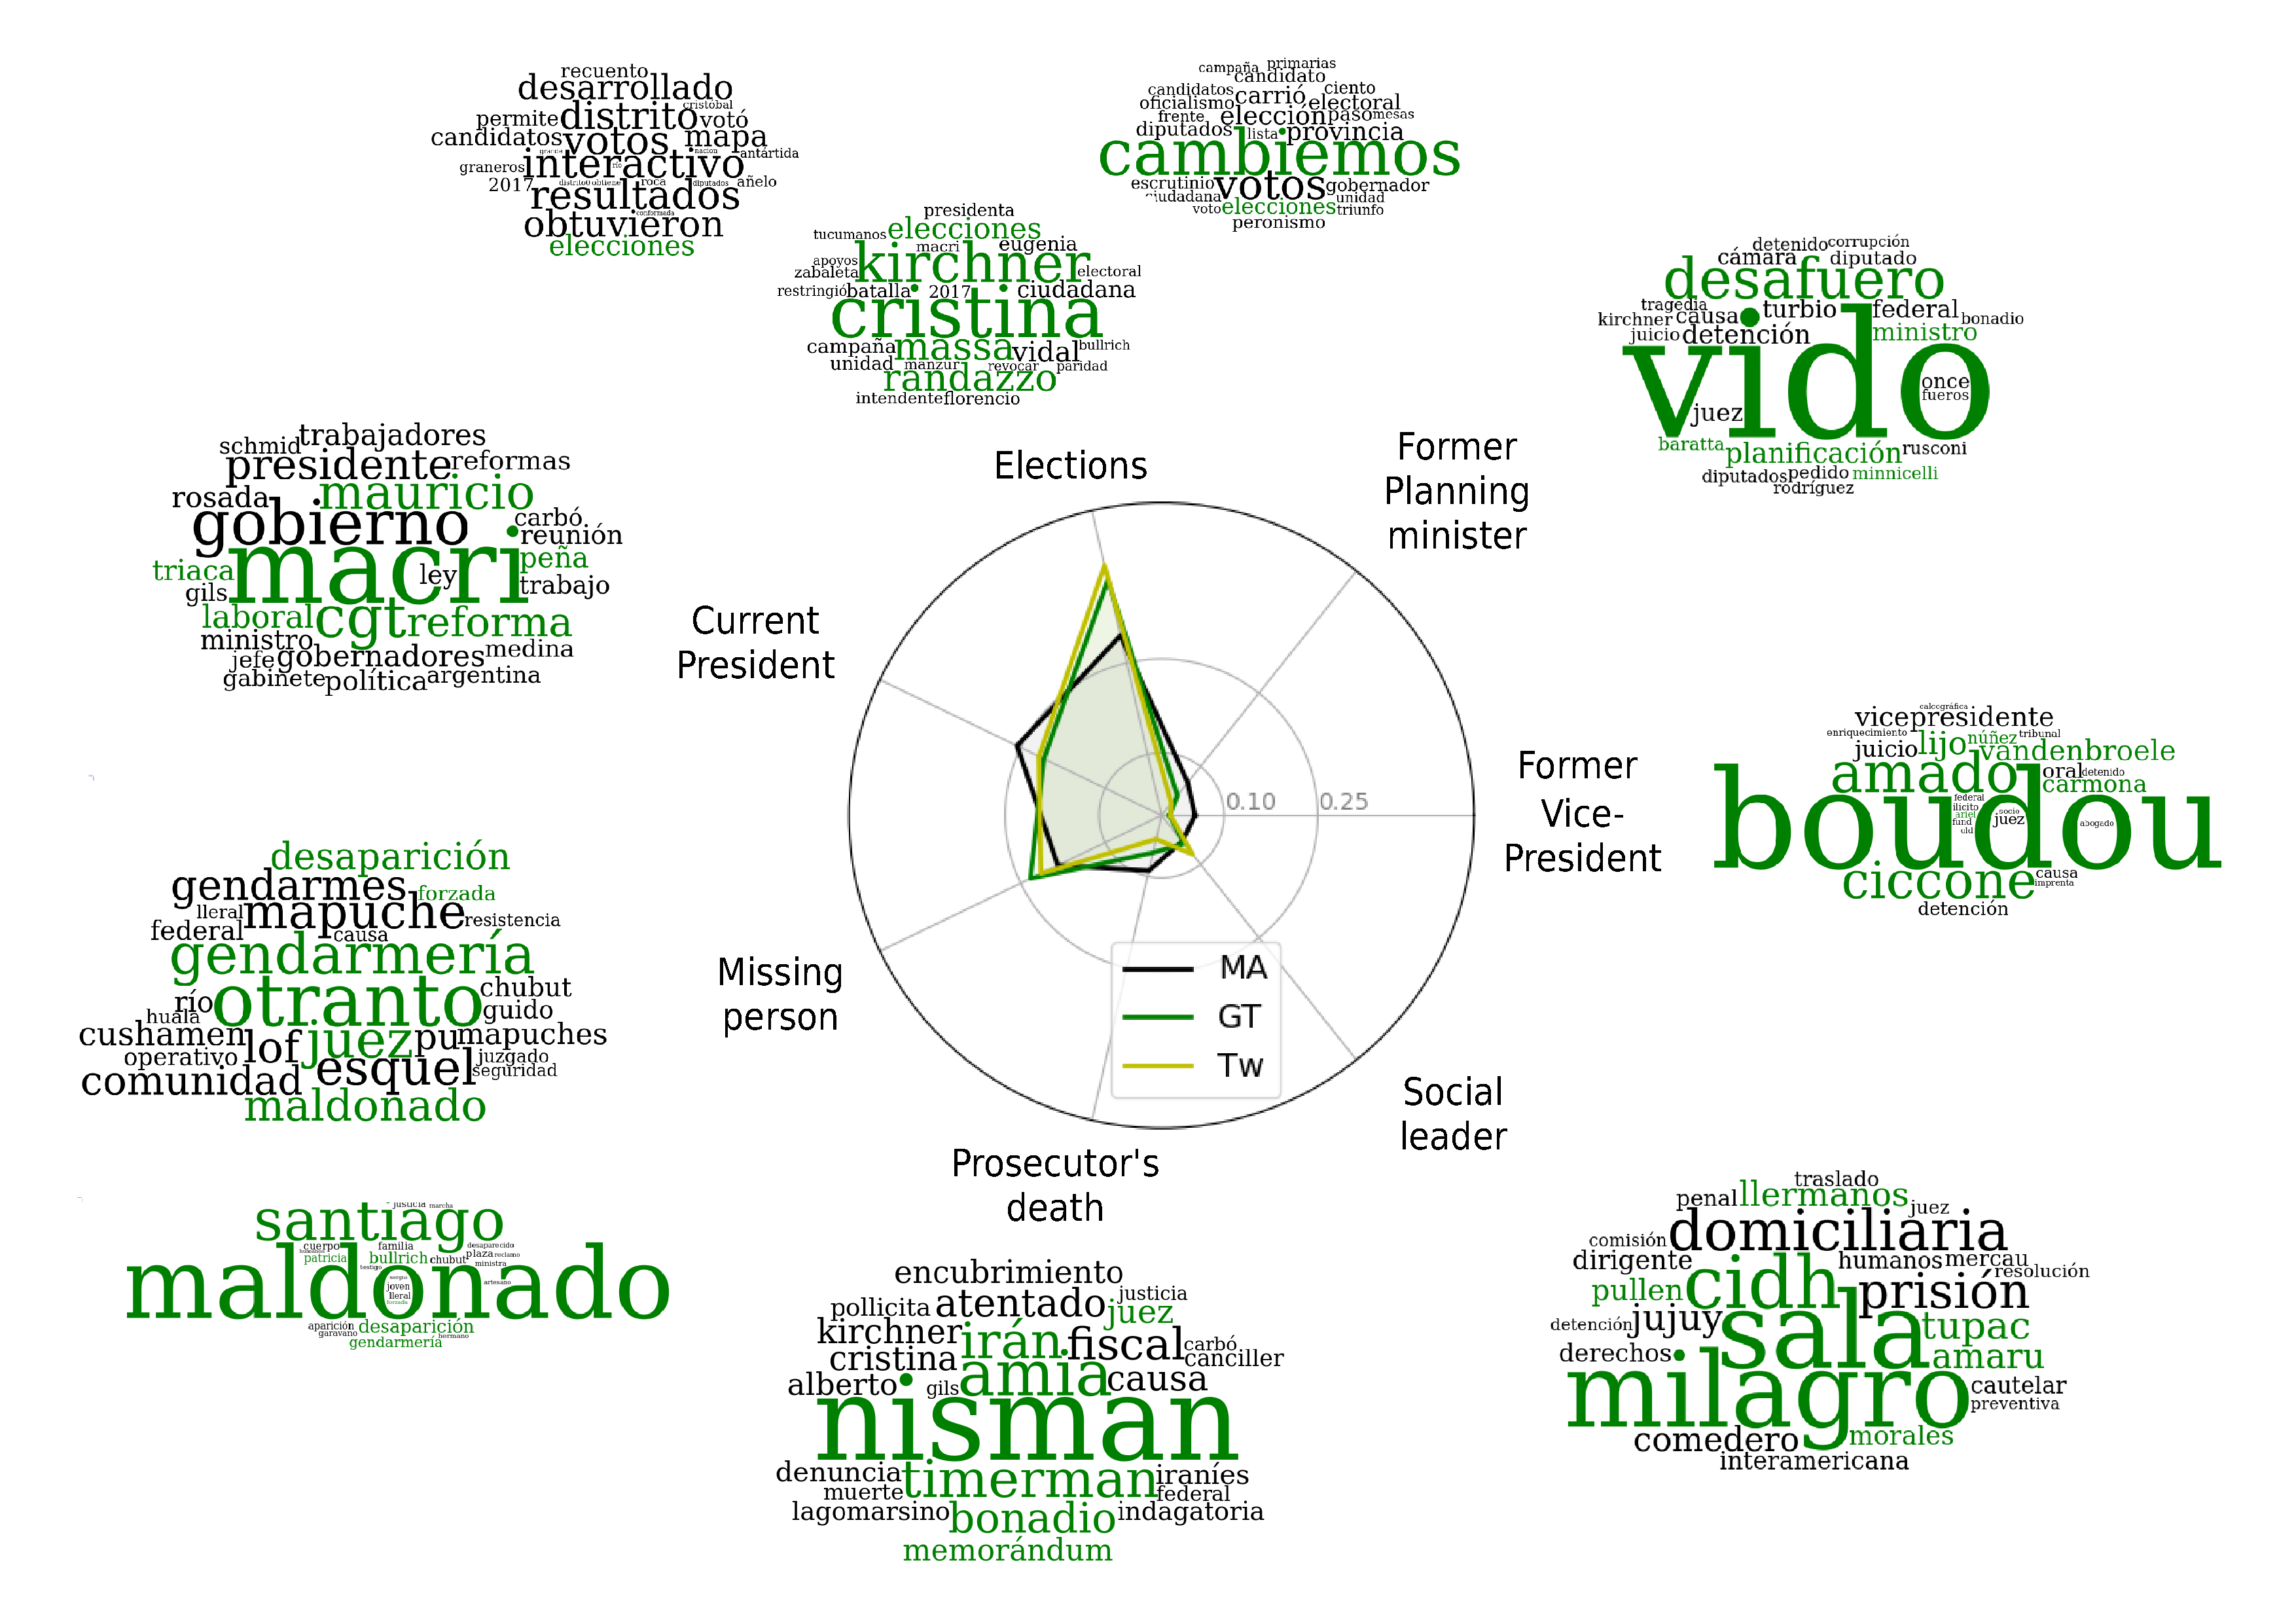
\includegraphics[width = \textwidth]{Fig1.pdf}
\caption{\textbf{Radar plots of the Media and Public Agendas represented by the ten topic (then collapsed to seven) distribution and their corresponding word clouds.} The Public Agenda is represented both by Google Trends (GT) and Twitter (Tw). Topic names are introduced together with the word clouds containing the most important keywords involved in the definition of each topic. In green color we show the keywords used to define the topics in the Google Trends and Twitter queries (see tables \ref{table:gt_queries} and \ref{table:tw_queries}) and therefore in our construction of the Public Agenda.}
\label{fig:topics_wordclouds}
\end{figure}

\begin{figure}[h!]
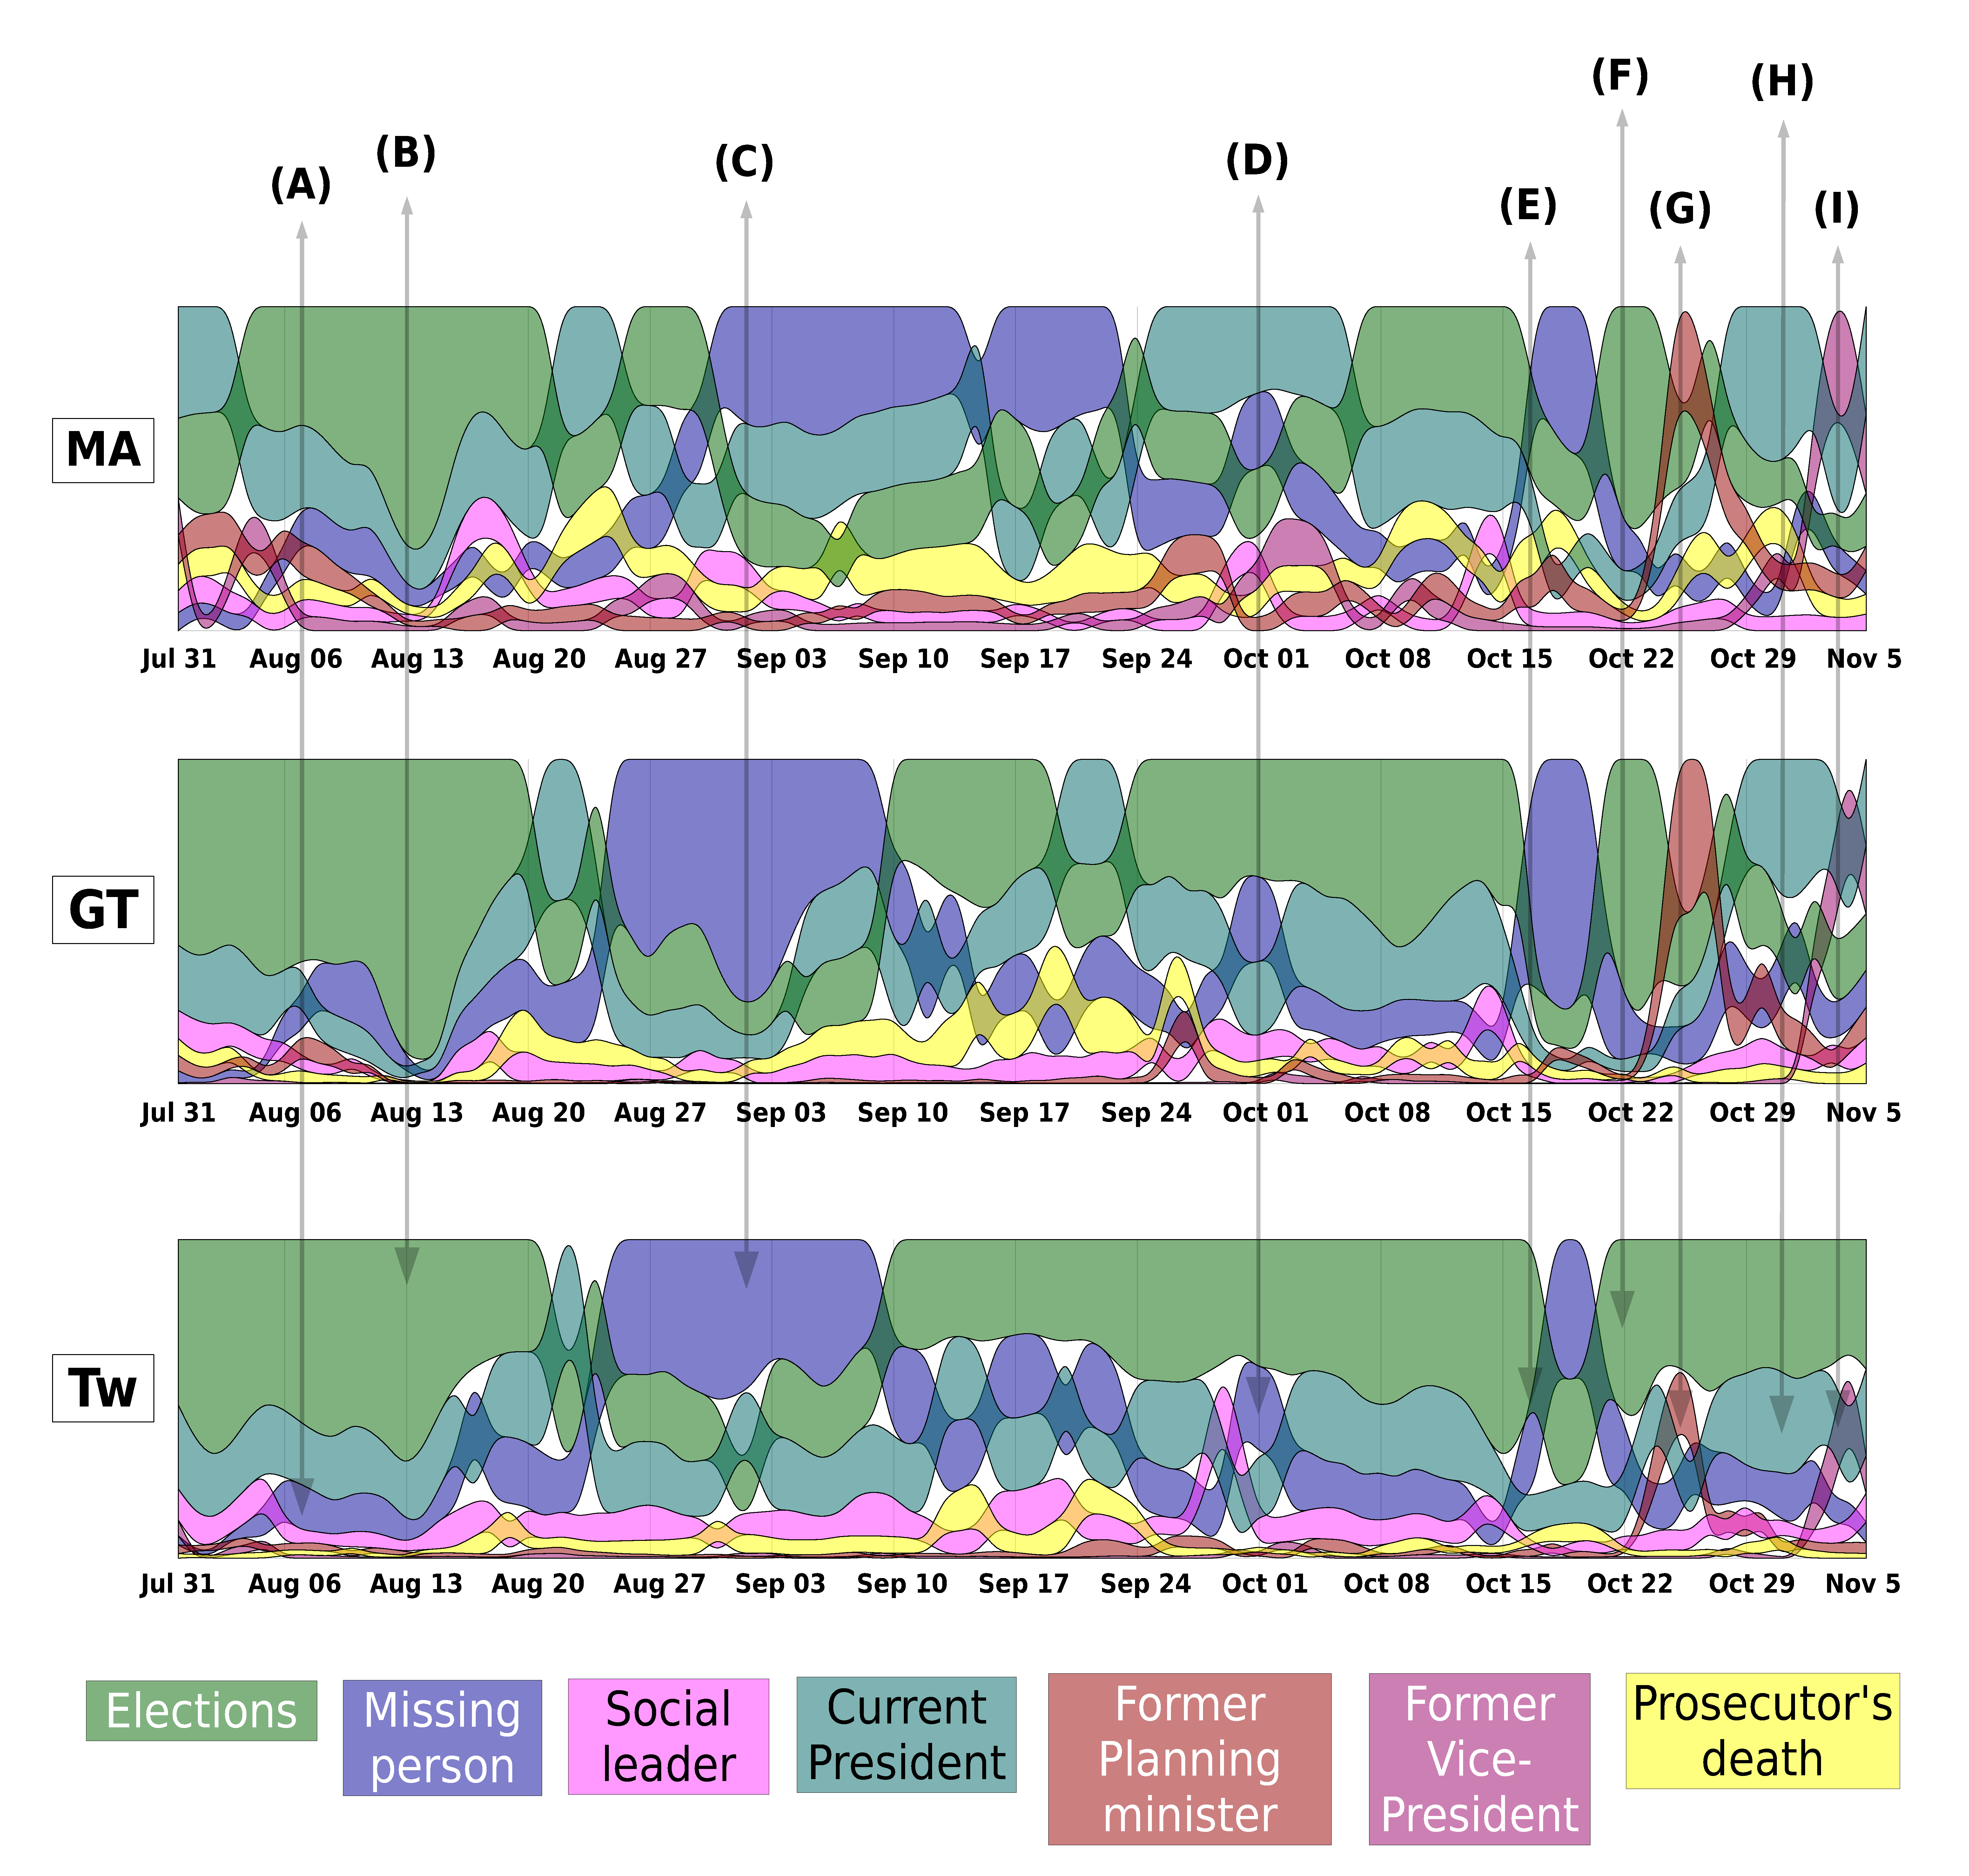
\includegraphics[width = \textwidth]{Fig2.pdf}
\caption{\textbf{Bump graph of the time-dependent Media (MA) and Public Agendas extracted from Google Trends (GT) and Twitter (Tw)}. Widths and rankings of the curves encode topic's relative weight. Also, some important events related to the topics are pointed out:
\textbf{A}: First news about Santiago Maldonado's disappearance (Missing person);
\textbf{B}: Primary elections;
\textbf{C}: March one month after Santiago Maldonado's disappearance;
\textbf{D}: March two months after Santiago Maldonado's disappearance;
\textbf{E}: Appearance of Santiago Maldonado's body;
\textbf{F}: General elections;
\textbf{G}: Julio De Vido's detention;
\textbf{H}: Debates on labor reform;
\textbf{I}: Amado Boudou's detention (Former vice-president).
A more detailed explanation is given in section \textbf{Supplementary Material}.}
\label{fig:all_agenda}
\end{figure}

\begin{figure}[h!]
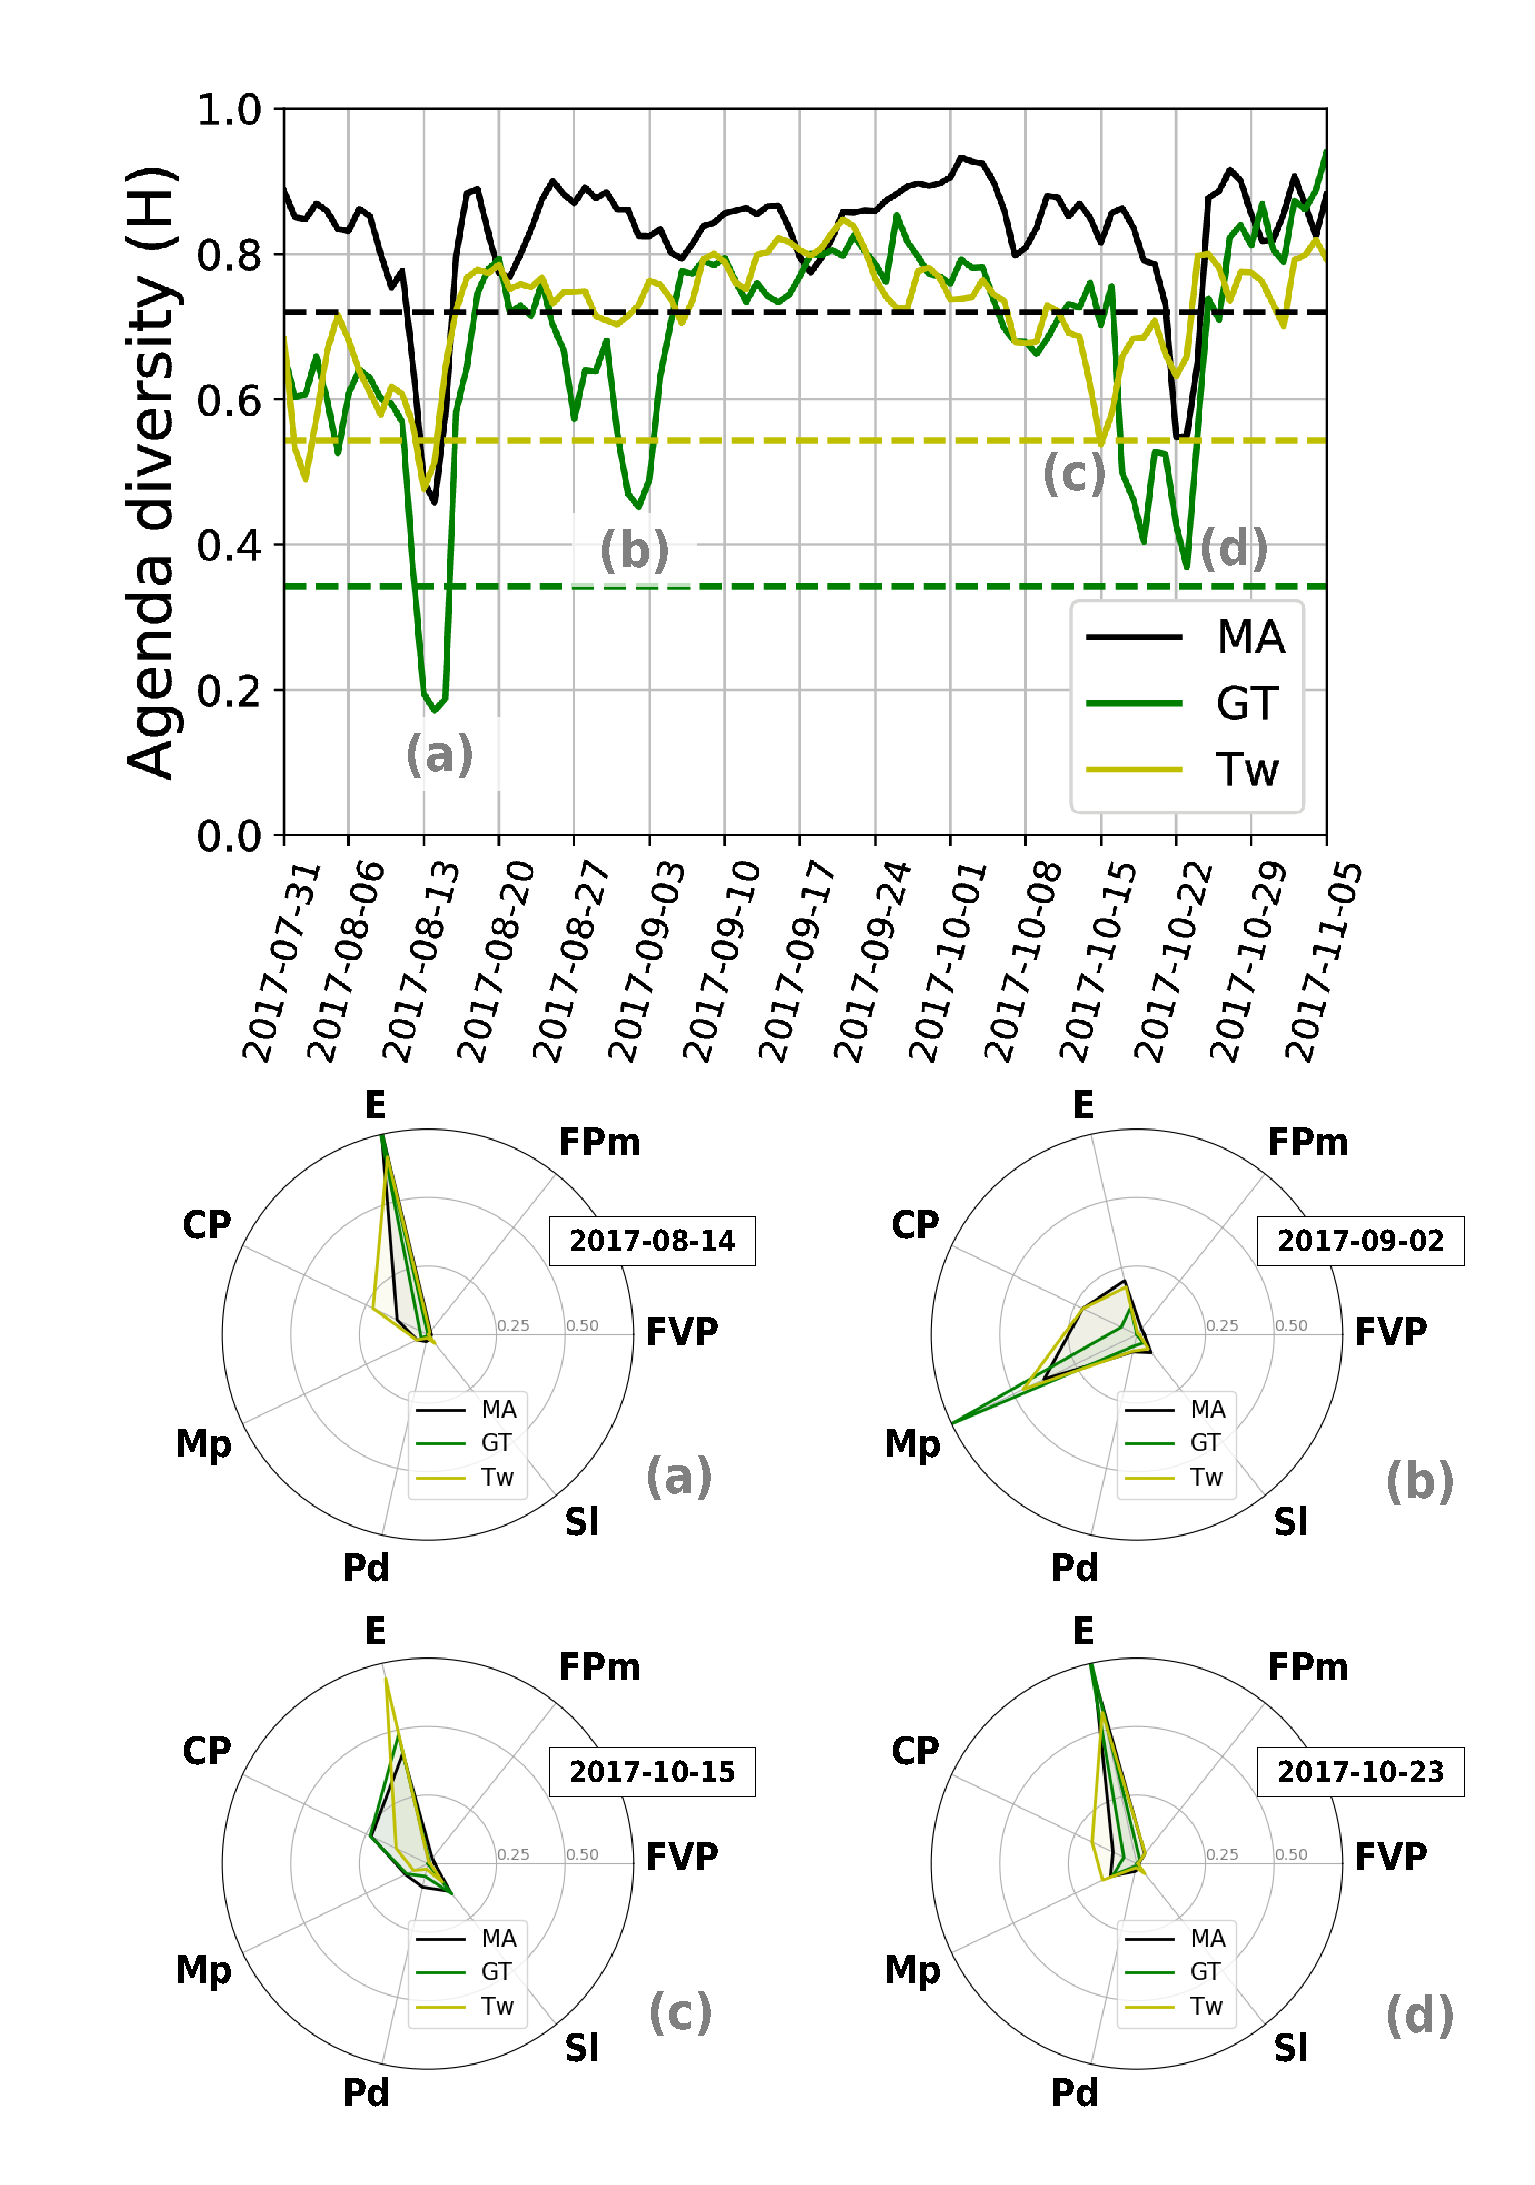
\includegraphics[height=0.7\textheight]{Fig3.pdf}
\caption{\textbf{Shannon entropy (H) as a measure of agenda diversity.} The Public Agenda shows a less diverse behavior than the Media Agenda as can be seen in the top figure. The horizontal lines correspond to the lower inner fences of each signal in order to identify outliers. The related radar plots show  the agenda at the selected days where the time series exhibit dropouts (points a-d), indicating that the most important topic catches most of the public's attention. \textbf{E}: Elections; \textbf{FPm}: Former Planning minister; \textbf{FVP}: Former Vice-President; \textbf{Sl}: Social leader; \textbf{Pd}: Prosecutor's death; \textbf{Mp}: Missing person; \textbf{CP}: Current President. }
\label{fig:shannon_entropy_agendas}
\end{figure}

\begin{figure}[h!]
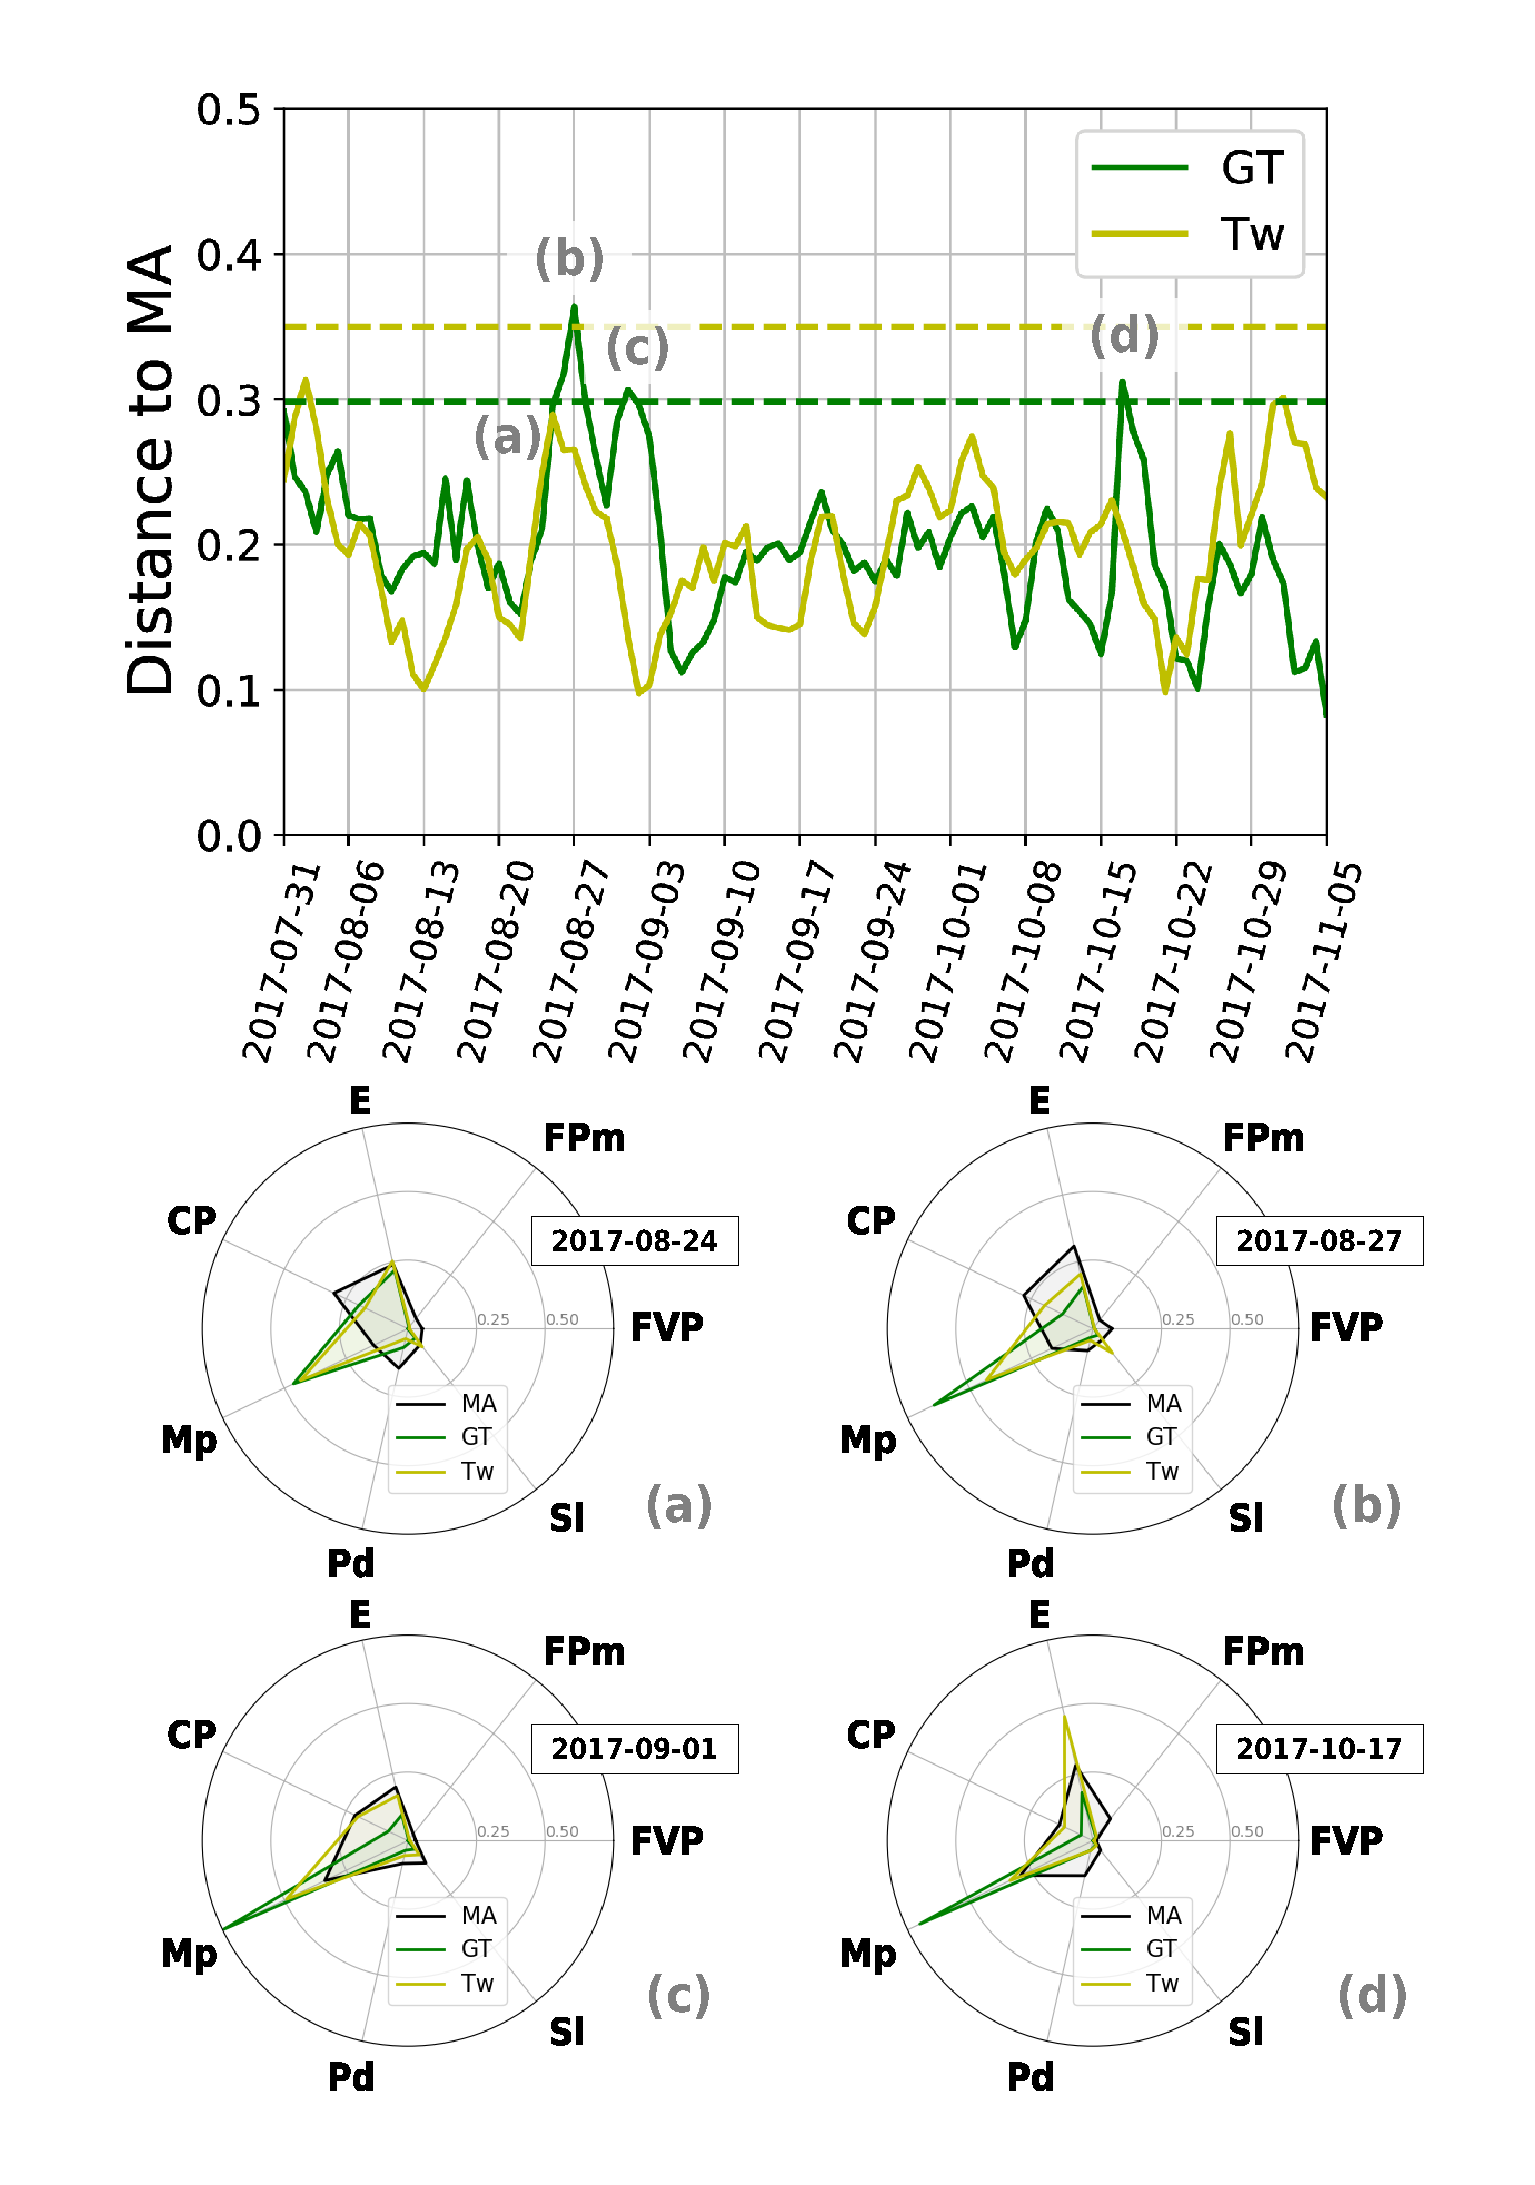
\includegraphics[height = 0.7\textheight]{Fig4.pdf}
\caption{\textbf{Jensen-Shannon distance between the Media and Public Agendas as a function of time} (with upper inner fences pointed out). Larger distances are due to a greater interest of the audience in the topic \emph{Missing person} which  decreases the interest in other topics. On the other side, the Media Agenda still keeps certain degree of diversity. \textbf{E}: Elections; \textbf{FPm}: Former Planning minister; \textbf{FVP}: Former Vice-President; \textbf{Sl}: Social leader; \textbf{Pd}: Prosecutor's death; \textbf{Mp}: Missing person; \textbf{CP}: Current President.}
\label{fig:jensen_shannon_gt}
\end{figure}

\begin{figure}[h!]
\includegraphics[width = \textwidth]{Fig5.pdf}
\caption{\textbf{Bump charts of newspaper agendas and radar plot of the average distributions.} The figure shows, in a qualitative way, the bias in the different newspaper agendas. For instance, the greater interest of \emph{P\'agina 12 (P12)} in the \emph{Missing person} topic and its slightly lower coverage in the \emph{Former Planning minister} respect to the other newspapers.}
\label{fig:news_agenda}
\end{figure}

\begin{figure}[h!]
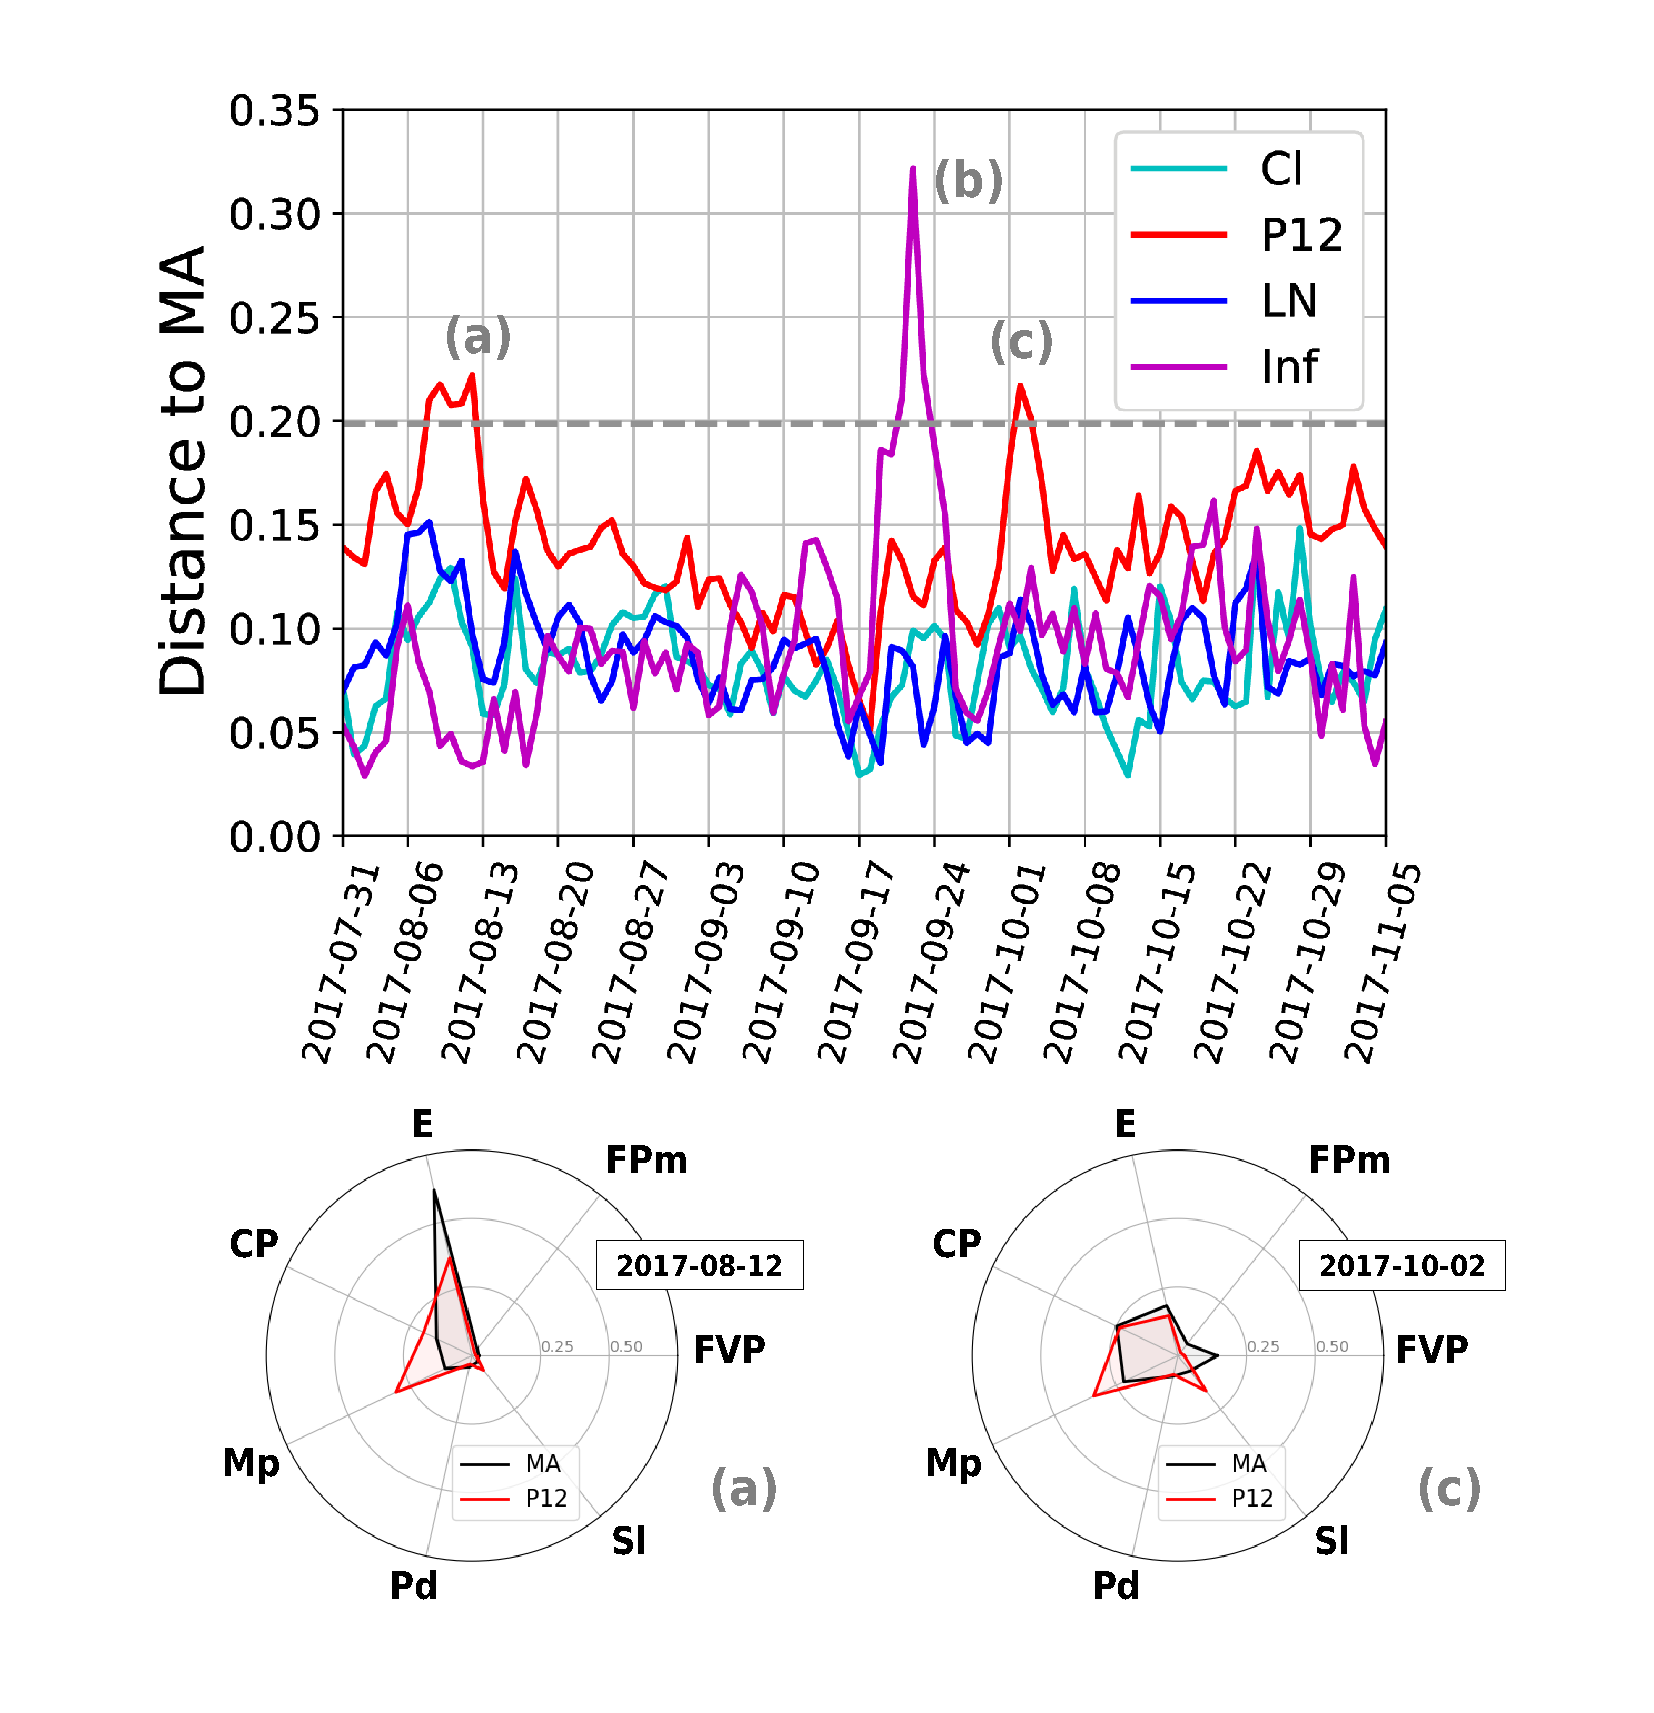
\includegraphics[width = \textwidth]{Fig6.pdf}
\caption{\textbf{Jensen-Shannon distance between the newspaper agendas and the Media Agenda as a function of time}. \emph{P\'agina 12} shows the most different behavior, motivated again by its interest in the \emph{Missing person} and \emph{Social leader} topics, as can be seen in the radar plots which belong to points (a) and (c). The anomalous behavior of \emph{Infobae} at point (b) is due to few articles around that date in our database, therefore we ignore its radar plot. \textbf{E}: Elections; \textbf{FPm}: Former Planning minister; \textbf{FVP}: Former Vice-President; \textbf{Sl}: Social leader; \textbf{Pd}: Prosecutor's death; \textbf{Mp}: Missing person; \textbf{CP}: Current President.}
\label{fig:jensen_shannon_news}
\end{figure}

\begin{figure}[h!]
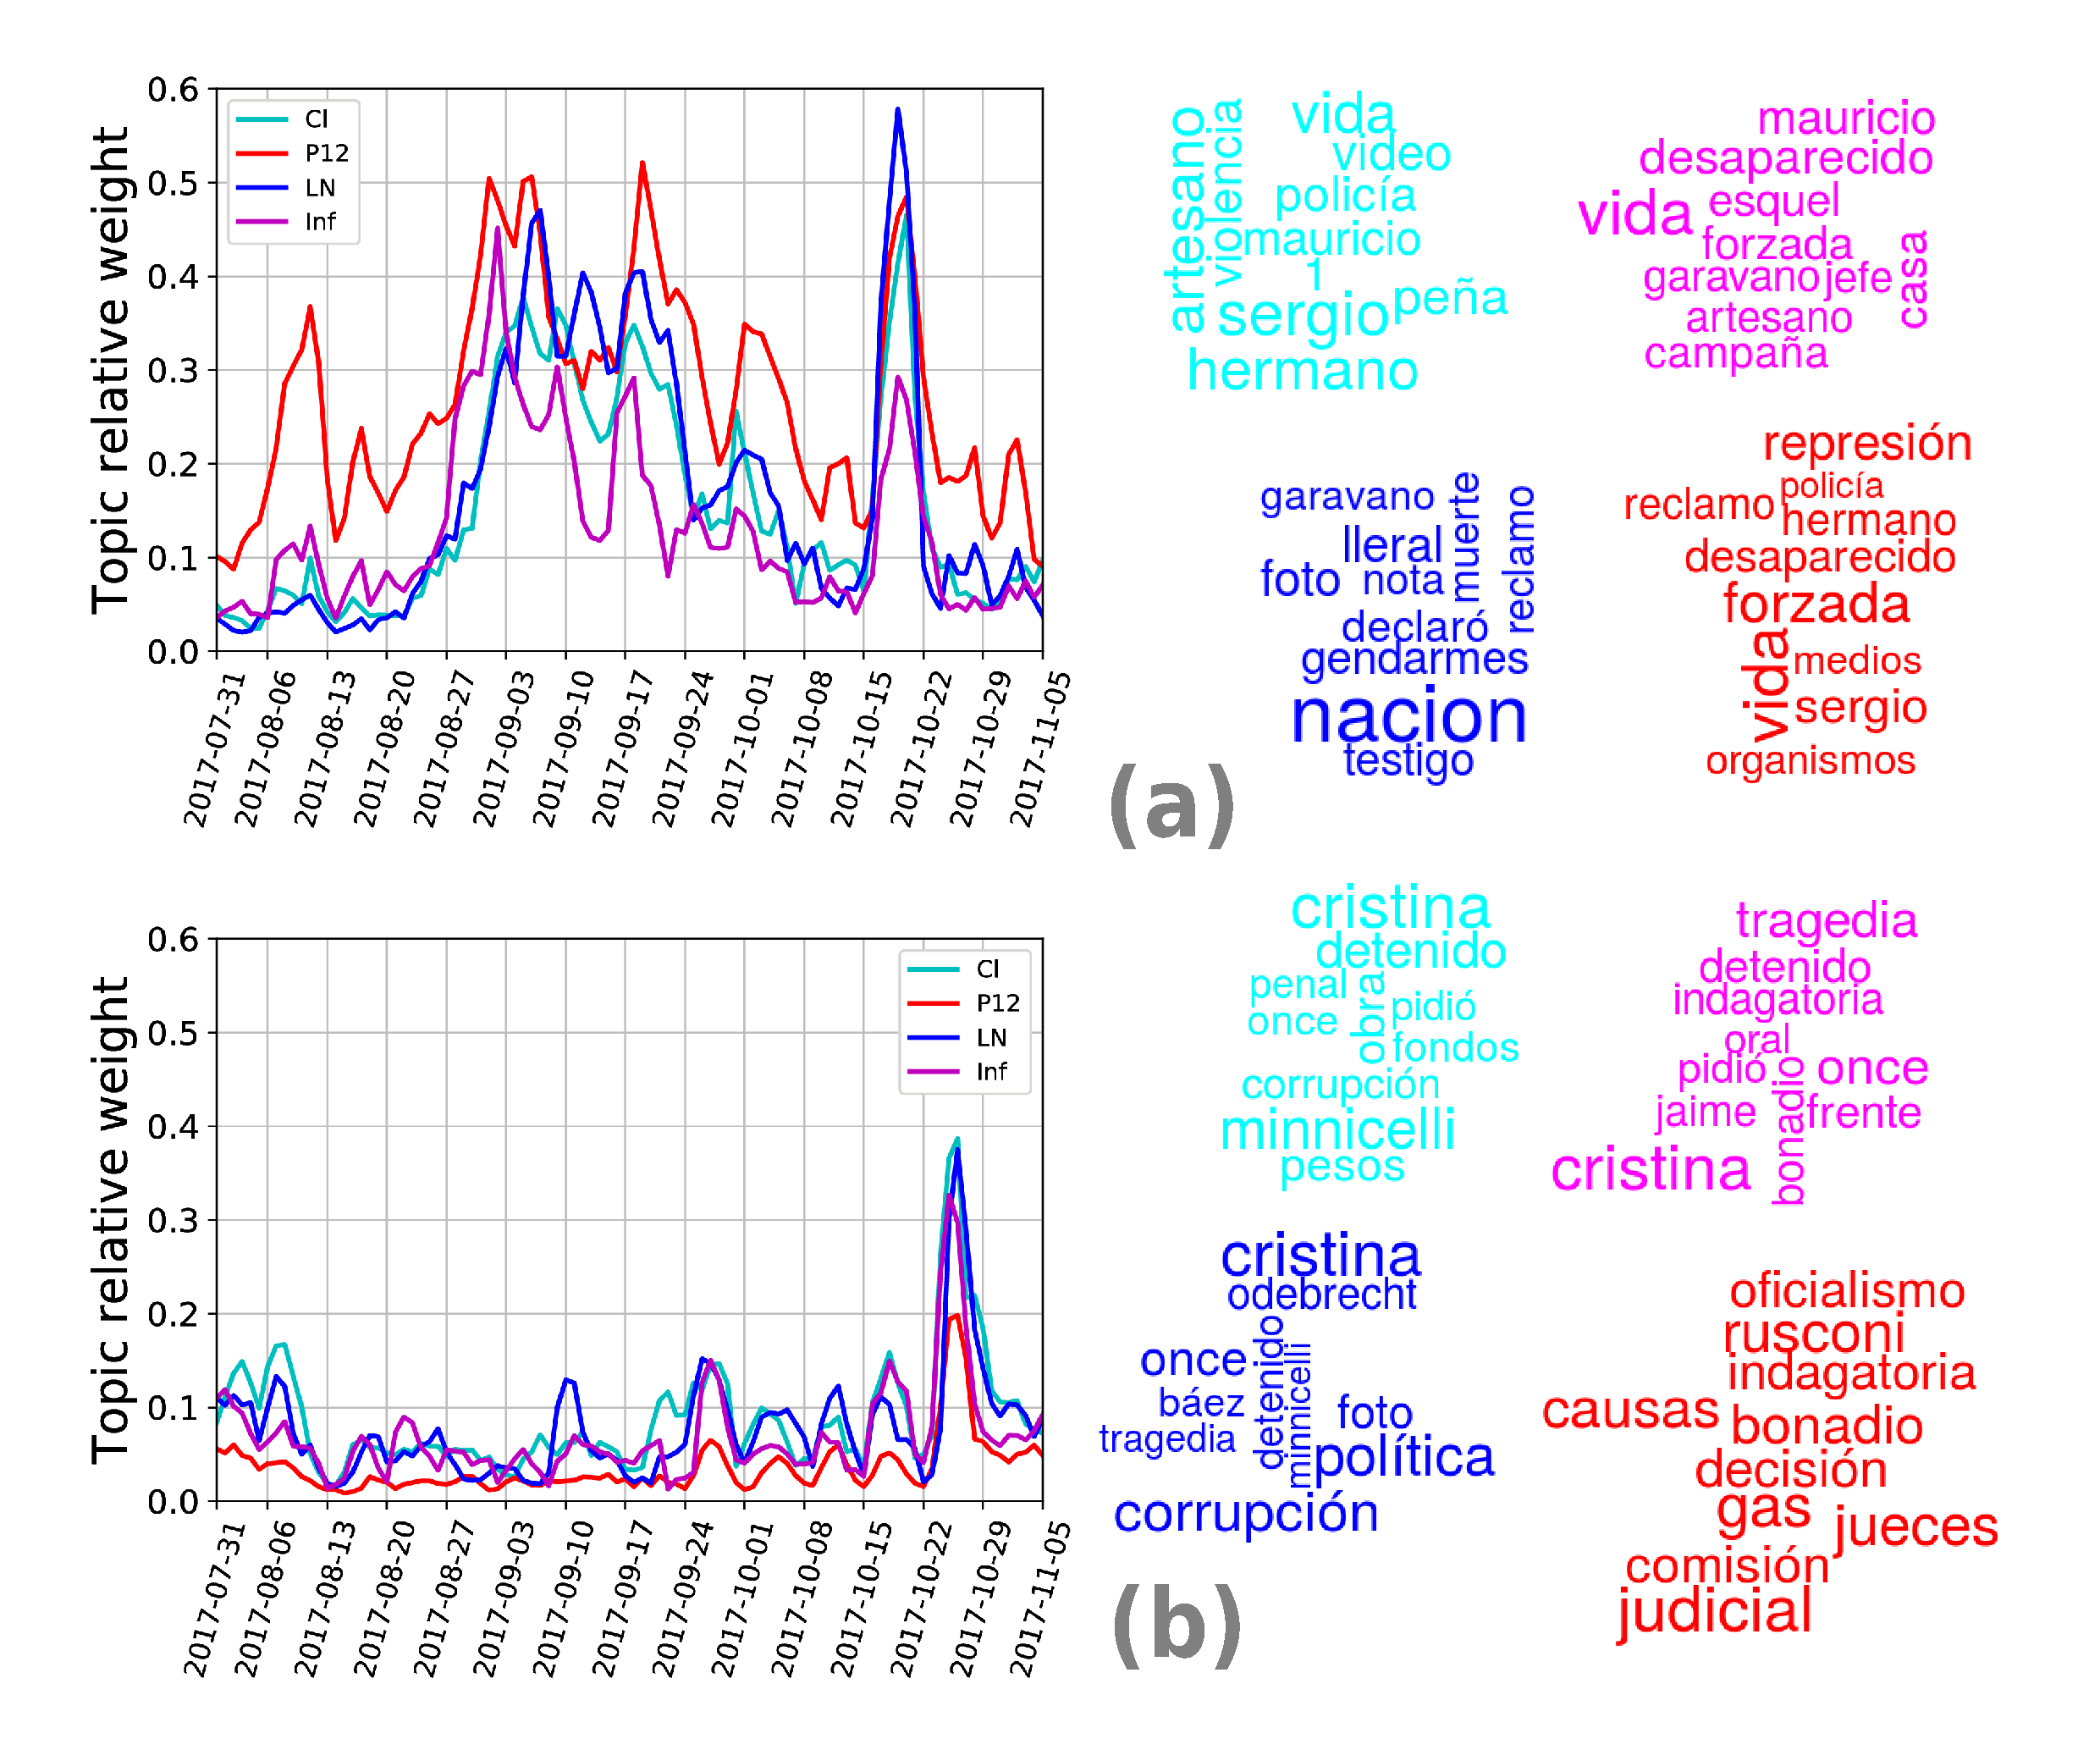
\includegraphics[width = \textwidth]{Fig7.pdf}
\caption{\textbf{Relative weight of the topics (a) \textit{Missing person}, and (b) \textit{Former Planning Minister}, and their corresponding word clouds of frequent newspaper keywords}. We interpreted the differences shown in given periods as an indicator of coverage bias. For instance, in figure (a) \emph{P\'agina 12} pays a greater attention in the first days. In the word-clouds, we show which of the defining words are more frequently used by the corresponding newspaper. Most of them are less informative, but others seem to represent a first approximation in the study of framing.}
\label{fig:topics_temporal_profiles}
\end{figure}

\begin{figure}[h!]
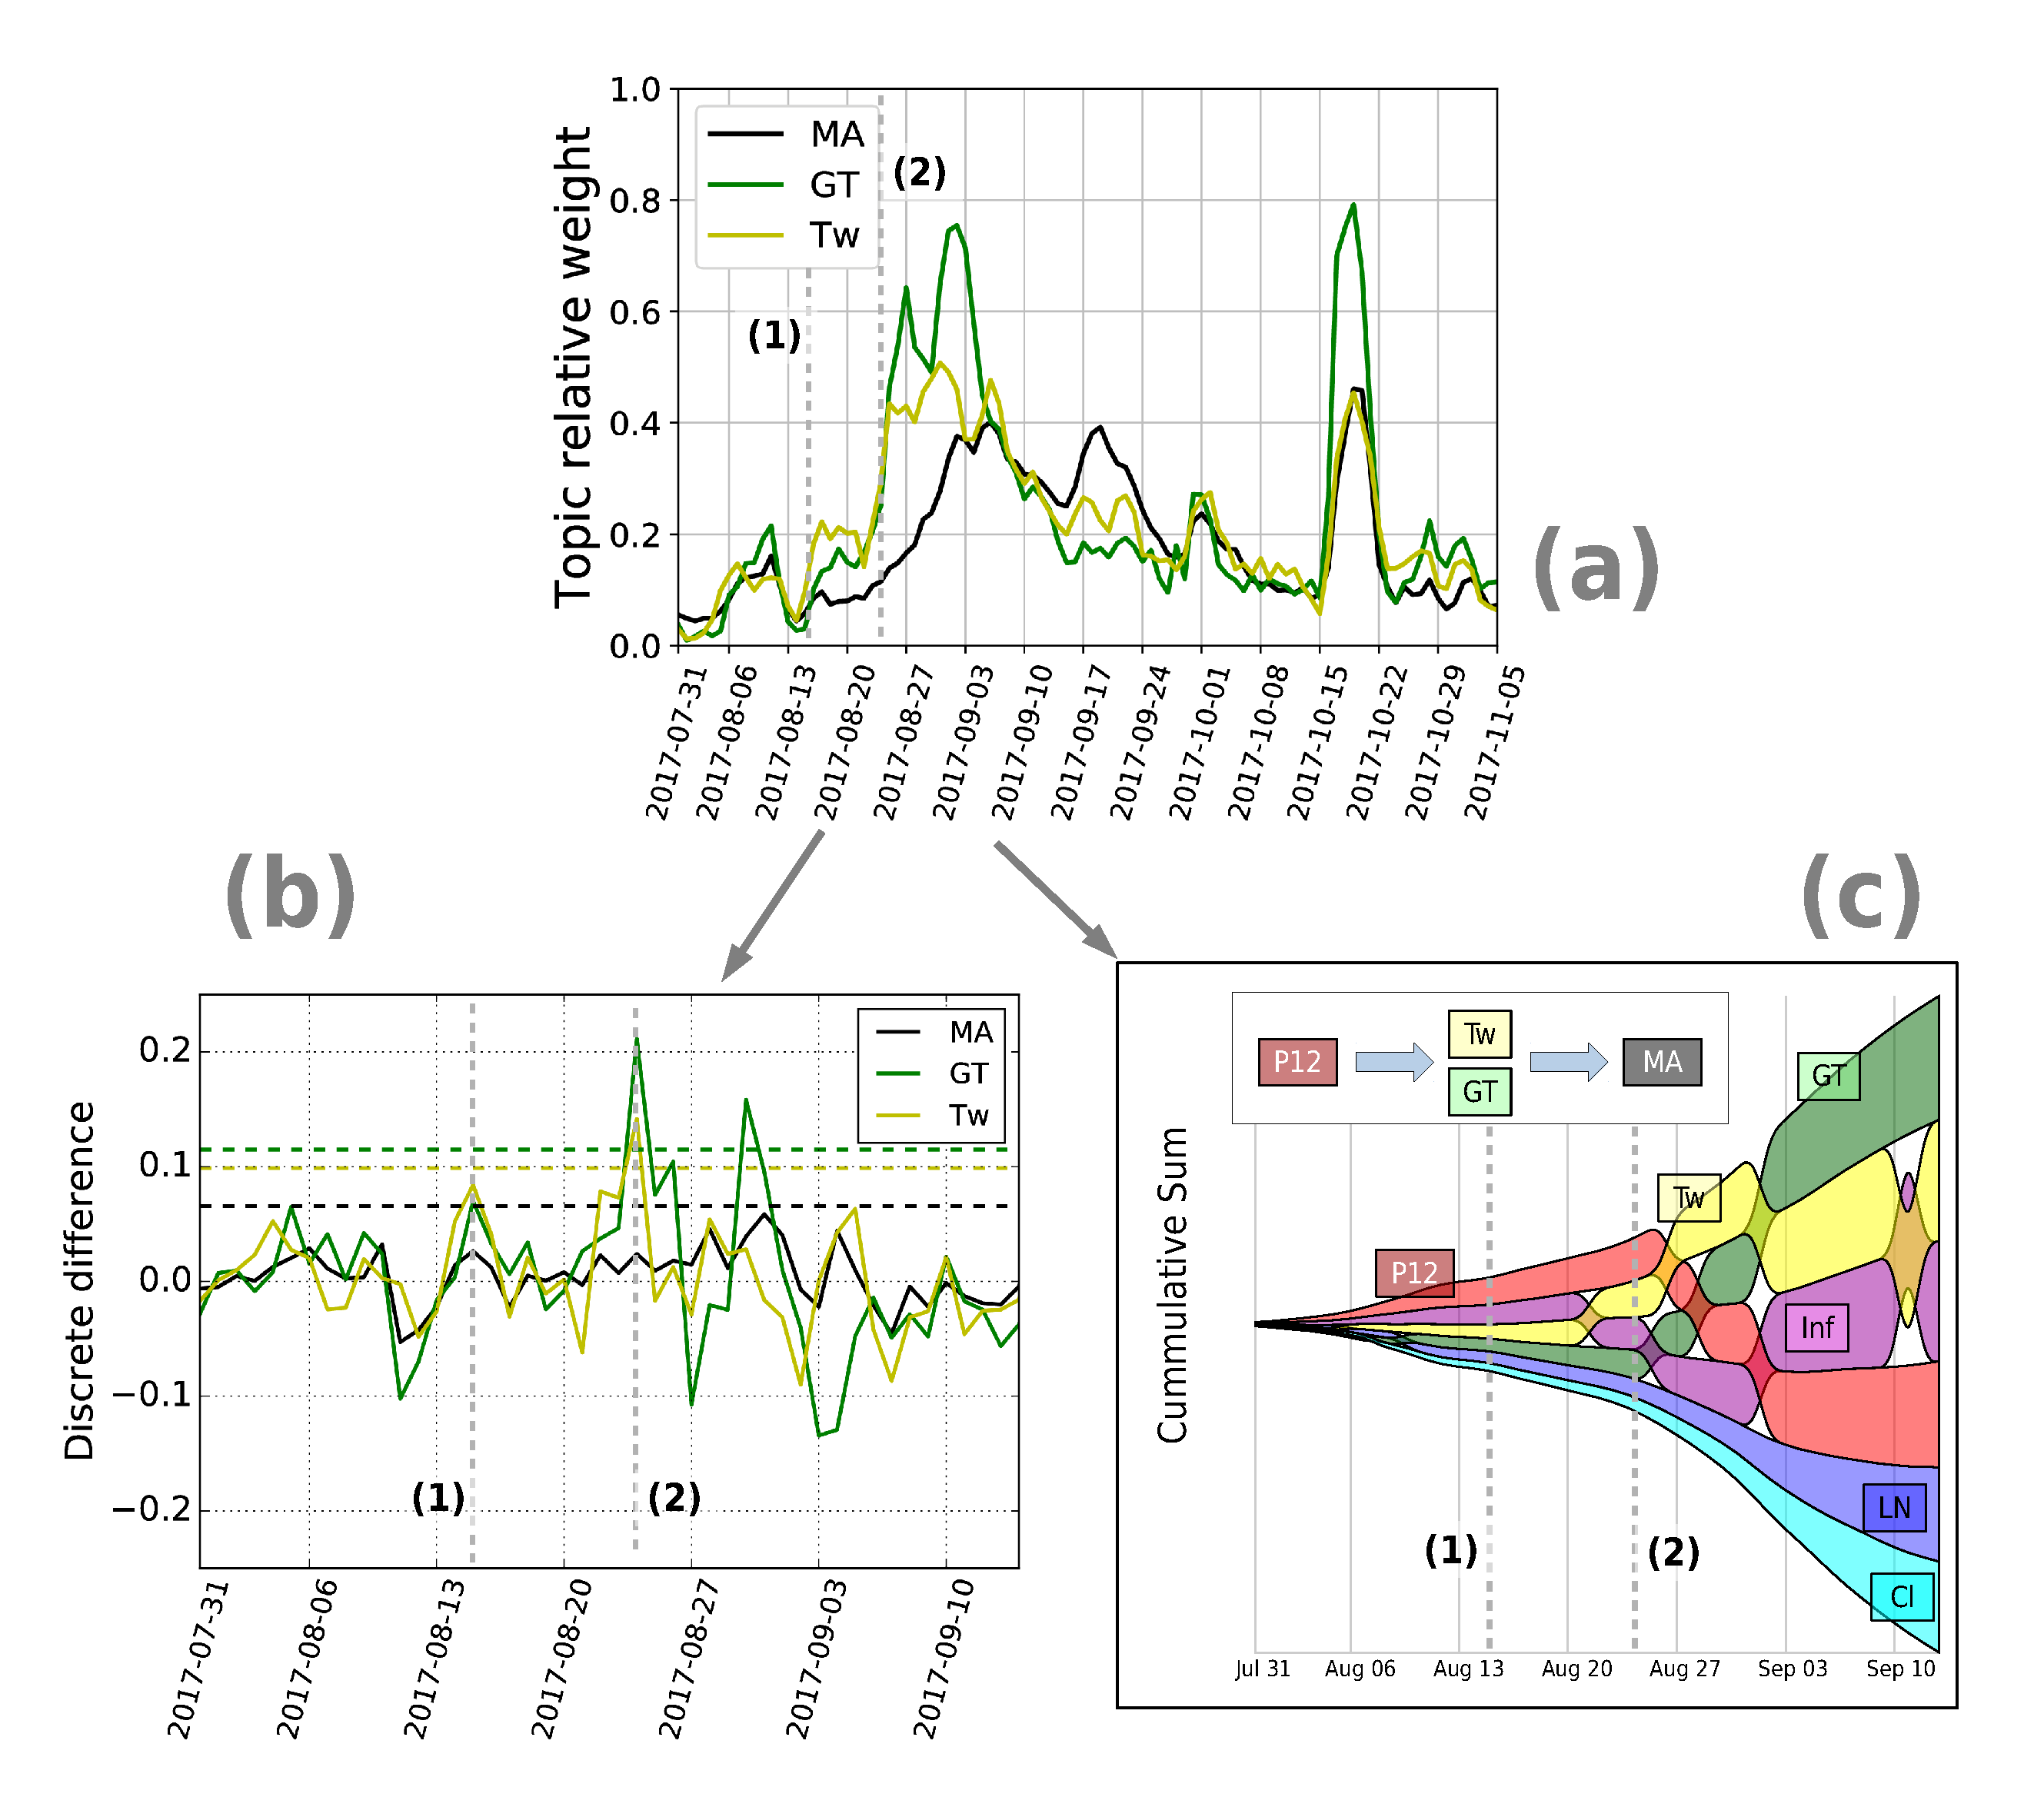
\includegraphics[width = \textwidth]{Fig8.pdf}
\caption{\textbf{Non-trivial agenda interplay in the Missing person topic.}
The temporal profiles of figure (a) show that the Public and Media agenda seem to differentiate around August 15th (vertical grey line (1)) and the Public increases abruptly its interest in the topic around August 24th (grey line (2)). It can be seen also in figure (b), where the discrete differences were computed. 
With the computing of the cumulative coverage of figure \ref{fig:topics_temporal_profiles} and figure (a), represented as a bump chart in figure (c), we suggest that the topic was first set by \emph{P\'agina 12} and then the audience interest causes the coverage of the rest of the media.
}
\label{fig:Maldonado_setagenda}
\end{figure}

\begin{figure}[h!]
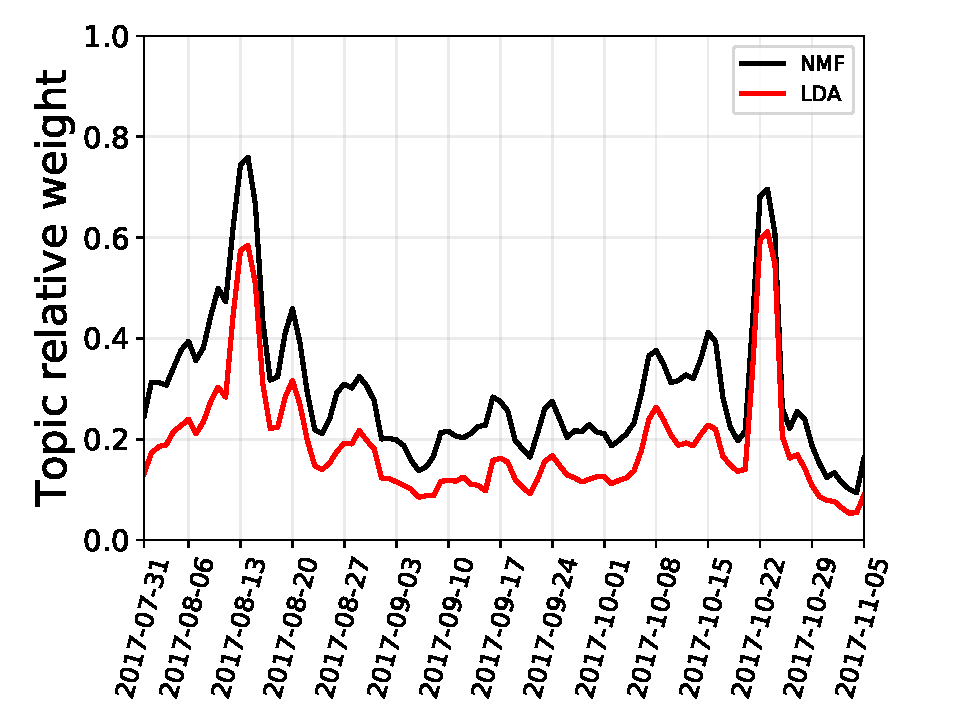
\includegraphics[scale = 0.3]{FigA2.pdf}
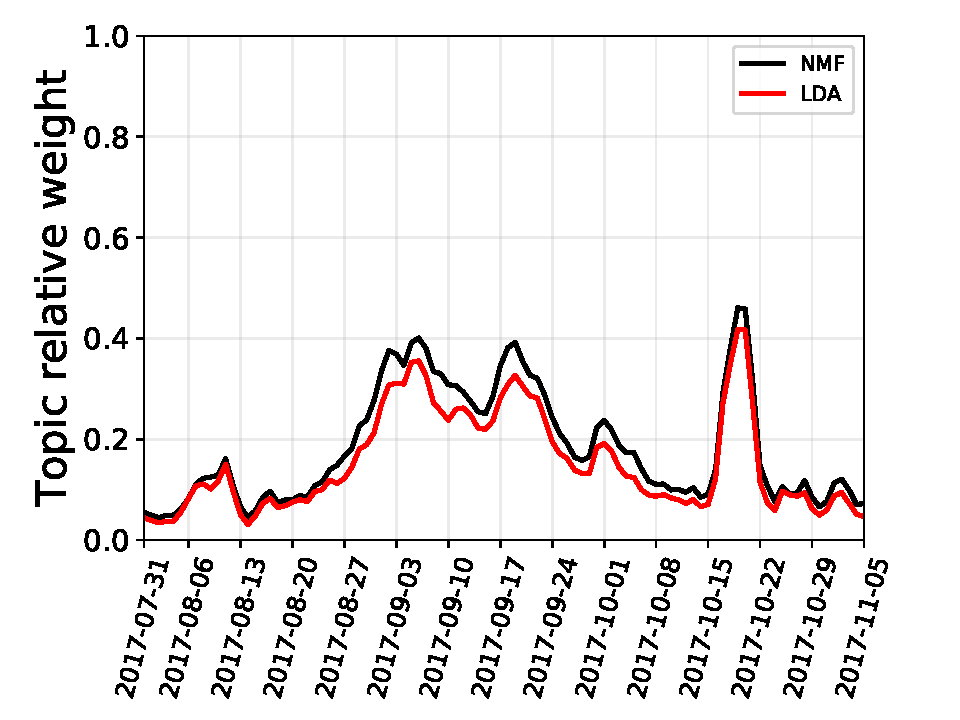
\includegraphics[scale = 0.3]{FigA1.pdf}
\caption{Temporal profiles of topics \emph{Elections} (left) and \emph{Missing Person} (right) for both LDA and NMF. All the topics found by applying NMF have a highly correlated counterpart in LDA.} 
\label{fig:temporal_profiles_nmf_lda}
\end{figure}

%%%%%%%%%%%%%%%%%%%%%%%%%%%%%%%%%%%
%%                               %%
%% Tables                        %%
%%                               %%
%%%%%%%%%%%%%%%%%%%%%%%%%%%%%%%%%%%

%% Use of \listoftables is discouraged.
%%
\section*{Tables}

\begin{table}[h!]
\caption{Queries used in Google Trends in order to build the Public Agenda.}
\begin{tabular}{l|p{7.5cm}}
Topic name & Google Trends query \\ \hline
Elections & elecciones + cambiemos + cristina kirchner + massa + randazzo \\
Missing person & santiago maldonado + juez otranto + patricia bullrich + gendarmería + desaparici\'on forzada \\
Former Planning minister & de vido + desafuero + ministro de planificaci\'on + minnicelli + baratta \\
Current President & mauricio macri + cgt + reforma laboral + peña + triaca \\
Social leader & milagro sala + cidh + tupac amaru + pullen llermanos + morales \\
Prosecutor's death & nisman + amia + memor\'andum con ir\'an + timerman + juez bonadio \\
Former Vice-President & amado boudou + ciccone + ariel lijo + vandenbroele + núñez carmona \\
\end{tabular}
\label{table:gt_queries}
\end{table}

\begin{table}[h!]
\caption{Queries used in Twitter: Due to different characteristics in the search tool of Twitter, we adapted the queries employed in Google Trends, but preserving, at least we can, the most important keywords.}
\begin{tabular}{l|p{7.5cm}}
Topic name & Twitter query \\ \hline
Elections & elecciones + cambiemos + kirchner + massa + randazzo \\
Missing person & maldonado + otranto + gendarmer\'ia + desaparici\'on \\
Former Planning minister & vido + desafuero + minnicelli + baratta \\
Current President & macri + cgt + laboral +  triaca \\
Social leader &  sala + cidh + tupac + amaru + pullen + llermanos + morales \\
Prosecutor’s death & nisman + amia + memorandum + timerman +  bonadio \\
Former Vice-President & boudou + ciccone +  lijo + vandenbroele + carmona \\ 
\end{tabular}
\label{table:tw_queries}
\end{table}


\begin{table}[h!]
\caption{Correlation between the topic temporal profiles of the Public Agenda and their counterpart in Media Agenda.
All correlation values are statistically significant ($p < 10^{-9}$), except (*) which is significant with $p < 0.05$.}
\begin{tabular}{lccc}
Topic name & Correlation MA and GT & MA and Tw & GT and Tw \\ \hline
Elections & \textbf{0.81} & \textbf{0.59} & \textbf{0.75} \\
Missing person & \textbf{0.68} & \textbf{0.76} & \textbf{0.89} \\
Former Planning minister & \textbf{0.92} & \textbf{0.82} & \textbf{0.87} \\
Current President & \textbf{0.77} & \textbf{0.75} & \textbf{0.63} \\
Social leader & \textbf{0.49} & \textbf{0.25(*)} & \textbf{0.57} \\
Prosecutor's death & \textbf{0.56} & \textbf{0.59} & \textbf{0.75} \\
Former Vice-President & \textbf{0.90} & \textbf{0.92} & \textbf{0.97}\\
\end{tabular}
\label{table:gt_all_correlation}
\end{table}

\begin{table}[h!]
\caption{Correlation between the temporal profiles of the topics found in NMF and associated topics in LDA.}
\begin{tabular}{lc}
Topic name & Correlation between NMF and LDA \\ \hline
Elections & \textbf{0.98} \\
Missing person & \textbf{0.99} \\
Former Planning minister + Former Vice-President & \textbf{0.89} \\
Current President & \textbf{0.94} \\
Social leader & \textbf{0.94} \\
Prosecutor's death & \textbf{0.83} \\
\end{tabular}
\label{table:correlation_nmf_lda}
\end{table}


%%%%%%%%%%%%%%%%%%%%%%%%%%%%%%%%%%%
%%                               %%
%% Additional Files              %%
%%                               %%
%%%%%%%%%%%%%%%%%%%%%%%%%%%%%%%%%%%

%\section*{Additional Files}
%  \subsection*{Additional file 1 --- Sample additional file title}
%    Additional file descriptions text (including details of how to
%    view the file, if it is in a non-standard format or the file extension).  This might
%    refer to a multi-page table or a figure.

%  \subsection*{Additional file 2 --- Sample additional file title}
%    Additional file descriptions text.


\end{backmatter}
\end{document}
